% =============================================================================
% GDF-Net: Breaking the Feedback Trap via Gradient Decoupling and
% Multi-Scale Feedback Attention for Biomedical Image Segmentation
%
% Formatted for IEEE Transactions on Medical Imaging (IEEEtran)
% =============================================================================
\documentclass[journal, 10pt]{IEEEtran}

% --- Graphics & Floats -------------------------------------------------------
\usepackage{graphicx}
\usepackage{float}
\usepackage{stfloats}       % improved two-column float placement (table*/figure*)
\usepackage{subcaption}
\usepackage{tikz}
\usetikzlibrary{positioning, arrows.meta, shapes.geometric}

% --- Math --------------------------------------------------------------------
\usepackage{amsmath, amssymb}
\usepackage{amsthm}
\newtheorem{theorem}{Theorem}
\newtheorem{lemma}{Lemma}

% --- Tables ------------------------------------------------------------------
\usepackage{booktabs}
\usepackage{multirow}
\usepackage{tabularx}
\usepackage{makecell}

% --- Fonts & Micro-typography ------------------------------------------------
\usepackage[T1]{fontenc}
\usepackage{lmodern}
\usepackage{microtype}

% --- Color, References, Hyperlinks -------------------------------------------
\usepackage{xcolor}
\usepackage{cite}
\usepackage[
  pagebackref=true,
  breaklinks=true,
  colorlinks,
  bookmarks=false,
  citecolor=blue,
  linkcolor=red,
  urlcolor=blue
]{hyperref}

% =============================================================================
\begin{document}

\title{GDF-Net: Breaking the Feedback Trap via Gradient Decoupling and Multi-Scale Feedback Attention for Biomedical Image Segmentation}

\author{%
  Nguyen~Nam~and~Co-Authors%
  \thanks{N.~Nam is with the Department of Computer Science and Biomedical Engineering. (Email: nghoofnam@gmail.com).}%
}

\maketitle

% -----------------------------------------------------------------------------
\begin{abstract}
Recurrent feedback architectures in biomedical vision are designed to iteratively refine ambiguous segmentation boundaries by feeding past prediction masks back into intermediate feature representations. However, canonical feedback networks---most notably the Feature Attention Network (FANet)---suffer from a severe, pervasive pathology: the \textit{Feedback Trap}. When prediction history serves simultaneously as forward spatial guidance and as an unconstrained backward optimization path, recursive gradient loops induce severe Batch Normalization drift, lock early encoder layers into hallucinated background noise, and cause runaway false-positive over-segmentation. In this paper, we conduct a rigorous mechanistic investigation into recurrent gradient dynamics and establish the \textbf{Feedback Firewall} principle: forward spatial guidance must be mathematically decoupled from backward gradient propagation ($\text{detach}(m^{(t-1)})$).

Building upon this theoretical principle, we introduce \textbf{GDF-Net} (Gradient-Decoupled Feedback Network), featuring: (1) a 4-channel input stem embedding detached prediction guidance with a learned spatial gate; (2) a pre-trained ResNet-34 transfer encoder; and (3) a Multi-scale Feedback Attention Decoder (MFAD) that modulates hierarchical features via continuous attention prior across all decoder resolutions. We validate GDF-Net across a comprehensive 7-dataset benchmark spanning endoscopy polyps (CVC-ClinicDB, Kvasir-SEG), electron microscopy cellular membranes (EM-Dataset), dermatological lesions (ISIC-2018), retinal vasculature (CHASE-DB1, DRIVE transfer), and fluorescent nuclei (DSB-2018). GDF-Net consistently surpasses original FANet baselines across 100\% of evaluated benchmarks: achieving \textbf{0.9427} Dice on CVC-ClinicDB (+4.69\,pp over baseline, beating paper best by +0.72\,pp), \textbf{0.9518} Dice on EM-Dataset (+17.02\,pp), \textbf{0.8880} Dice on Kvasir-SEG (+0.28\,pp), \textbf{0.9000} Dice on ISIC-2018 (+2.69\,pp), and slashing false positive rates by \textbf{65\%} on CHASE-DB1 (FPR down to 0.74\%). Furthermore, our forensic audit resolves historical inconsistencies in the literature, demonstrating that identical performance across feedback steps ($B_1 \equiv B_4$) in prior published tables stemmed from dormant feedback loops, while prolonged 500-epoch training induced catastrophic representation degradation. GDF-Net restores genuine iterative refinement and provides a sound, generalizable foundation for recurrent medical image segmentation.
\end{abstract}

\begin{IEEEkeywords}
Recurrent Feedback, Gradient Decoupling, Feedback Firewall, Medical Image Segmentation, Feedback Trap, Multi-scale Attention Decoder, GDF-Net, MFAD.
\end{IEEEkeywords}

% -----------------------------------------------------------------------------
% SECTIONS
% -----------------------------------------------------------------------------
\section{Introduction}
\label{sec:intro}

Biomedical image segmentation constitutes a fundamental cornerstone of computer-assisted intervention, pathological screening, and automated diagnosis~\cite{litjens2017survey, ronneberger2015unet}. In high-stakes clinical tasks---ranging from early endoscopic detection of precancerous colorectal polyps~\cite{siegel2023colorectal, jha2020kvasir, bernal2017comparative} and dermatological melanoma excision~\cite{codella2019skin} to retinal vascular micro-aneurysm grading~\cite{hoover2000locating, staal2004ridge} and cellular ultrastructure tracing~\cite{cardona2010integrated, caicedo2019nucleus}---accurate delineation of target boundaries is paramount. Automated systems must reliably discern ambiguous tissue interfaces, handle extreme shape heterogeneity, and suppress deceptive background artifacts under severe class imbalance.

To address complex and ill-defined boundaries, deep architectures have increasingly incorporated \textbf{recurrent feedback mechanisms}~\cite{tomar2021fanet, liang2015recurrent, alom2018recurrent, tomar2021ddanet}. The foundational intuition of recurrent feedback is inspired by the human visual cortex: biological vision relies heavily on top-down iterative processing, where higher-level semantic interpretations recursively constrain and refine lower-level sensory feature representations~\cite{gilbert2013top, kietzmann2019recurrence}. A prominent pioneer in biomedical vision is the Feature Attention Network (FANet)~\cite{tomar2021fanet}, which introduced a multi-pass feedback loop. In FANet, past prediction masks ($m^{(t-1)}$) generated at feedback step $t-1$ are recursively re-injected into intermediate encoder-decoder feature maps via a spatial gating module (\texttt{MixPool}). In theory, this recurrent refinement process should iteratively suppress false positives, sharpen ambiguous object contours, and recover subtle morphological details.

\subsection{The Empirical Dilemma: The Feedback Trap and Representation Collapse}
Despite this compelling theoretical premise, practical deployment of recurrent feedback architectures in medical vision reveals a severe, paradoxical pathology: \textbf{chronic false-positive over-segmentation and optimization instability}. In clinical cohorts, qualitative and quantitative audits demonstrate that unconstrained feedback networks frequently exhibit severe prediction bleed, projecting masks tens of pixels beyond genuine anatomical boundaries into healthy parenchyma and background tissue. 

More critically, while modern loss engineering (e.g., asymmetric Tversky loss~\cite{salehi2017tversky} or boundary-weighted losses~\cite{kervadec2019boundary}) reliably curbs false positives in feedforward architectures, its optimization efficacy is completely neutralized once recurrent feedback is engaged. The network becomes trapped in an echo chamber of its own past predictions. 

Through rigorous representational and gradient audits, we identify the mathematical root cause of this failure, which we term the \textbf{Feedback Trap}. The core failure stems from a structural design flaw in conventional recurrent feedback: \textbf{forcing historical predictions to serve simultaneously as forward spatial guidance and as an unconstrained backward optimization path}. In canonical FANet~\cite{tomar2021fanet}, the spatial gating operator combines learnable internal attention ($\text{fmask}$) with downsampled recurrent feedback ($m_{\text{fg}}$) through hard binary gating:
\begin{equation}
  \label{eq:hard_gate_intro}
  \text{keep}_{\text{hard}} = \max\left(\mathbb{I}(\text{fmask} > 0.5),\; m_{\text{fg}}\right).
\end{equation}
This formulation triggers two structural failures:
\begin{enumerate}
  \item \textbf{Gradient Paralysis of Internal Attention:} Because the indicator function $\mathbb{I}(\cdot > 0.5)$ has a derivative of zero almost everywhere, $\frac{\partial \text{keep}}{\partial \text{fmask}} \equiv 0$. Consequently, the convolutional sub-networks tasked with extracting attention receive zero direct gradient signal from the downstream segmentation loss.
  \item \textbf{Toxic Recursive Backpropagation and Error Amplification:} Concurrently, non-zero gradients backpropagate unconstrained through the recurrent mask branch ($m_{\text{fg}}$). When the network generates an initial false positive, that erroneous prediction is re-injected as a spatial prior in subsequent iterations. Because the backward pass calculates gradients through this recursive dependency graph, early encoder representations experience massive Batch Normalization drift, feature variance collapses, and the model optimizes itself to justify its own prior hallucinations rather than ground-truth anatomy.
\end{enumerate}

Furthermore, our forensic re-examination of the literature reveals a stark historical anomaly: in Table~IX of the seminal FANet paper~\cite{tomar2021fanet}, reported test scores across feedback steps ($B_1 \to B_4$) are perfectly identical across multiple datasets. This mathematical identity demonstrates that in previous implementations, the feedback mechanism was effectively \textbf{dormant} in evaluation, or when trained for excessive cycles (500 epochs), degenerated into uncontrolled over-segmentation.

\subsection{The Solution: Gradient Decoupling and GDF-Net}
To resolve this fundamental pathology, we formulate the \textbf{Feedback Firewall} principle:
\begin{center}
  \textit{Forward spatial guidance must be mathematically decoupled from backward gradient propagation.}
\end{center}
By enforcing a strict stop-gradient operator on recurrent predictions ($\text{detach}(m^{(t-1)})$), historical predictions act strictly as clean forward spatial guidance, completely eliminating recursive error amplification in the backward pass.

Building upon this principle, we introduce \textbf{GDF-Net} (Gradient-Decoupled Feedback Network), an enhanced architecture that unifies three core innovations:
\begin{enumerate}
  \item \textbf{Decoupled Spatial Guidance Stem:} A 4-channel input convolutional stem that ingests both the original image and a detached prediction prior modulated by a learned spatial gate ($\sigma(\mathcal{W}_{\text{gate}} \cdot \text{detach}(m^{(t-1)}))$).
  \item \textbf{Multi-Scale Feedback Attention Decoder (MFAD):} Instead of confining feedback modulation to a single point, MFAD integrates hierarchical attention gates across all decoder skip connections, modulating intermediate features via continuous spatial priors: $\mathbf{F}_\ell \odot (1 + \mathcal{A}_\ell(\mathbf{m}_{\text{guide}}))$.
  \item \textbf{Universal Benchmark Validation Across 7 Modalities:} A rigorous, reproducible experimental protocol validating GDF-Net across 7 diverse biomedical datasets (CVC-ClinicDB, EM-Dataset, Kvasir-SEG, ISIC-2018, CHASE-DB1, DRIVE transfer, and DSB-2018).
\end{enumerate}

\subsection{Summary of Contributions}
The contributions of this work are summarized as follows:
\begin{enumerate}
  \item \textbf{Theoretical Diagnosis of the Feedback Trap:} We provide the first systematic mathematical formulation and empirical demonstration of the Feedback Trap in recurrent vision networks, diagnosing internal attention gradient paralysis and backward recursive error amplification.
  \item \textbf{The Feedback Firewall \& GDF-Net Architecture:} We establish the Gradient Decoupling principle and propose GDF-Net, integrating a 4-channel decoupled guidance stem with a Multi-scale Feedback Attention Decoder (MFAD) to enable stable, multi-resolution feature modulation.
  \item \textbf{Comprehensive 7-Dataset Benchmark Superiority:} We evaluate GDF-Net on 7 benchmark datasets across 4 distinct biomedical imaging domains. GDF-Net outperforms original FANet baselines across 100\% of evaluated benchmarks, achieving \textbf{0.9427} Dice on CVC-ClinicDB (+4.69\,pp), \textbf{0.9518} on EM-Dataset (+17.02\,pp), \textbf{0.8880} on Kvasir-SEG (+0.28\,pp), \textbf{0.9000} on ISIC-2018 (+2.69\,pp), \textbf{0.8953} on DSB-2018 (+2.32\,pp), \textbf{0.7932} on DRIVE (+3.14\,pp), and slashing false positive rates by \textbf{65\%} on CHASE-DB1.
  \item \textbf{Empirical Audit and Reproducibility:} We resolve the historical Table~IX discrepancy in the literature, demonstrating that true recurrent refinement is unlocked only under gradient decoupling, and provide verified, reproducible open-source implementations for all benchmarks.
\end{enumerate}

\section{Related Work}
\label{sec:related}

% -----------------------------------------------------------------------------
\subsection{Biomedical Image Segmentation}
Biomedical image segmentation encompasses diverse clinical imaging modalities with distinct visual and structural properties~\cite{litjens2017survey}. Beginning with the foundational U-Net architecture~\cite{ronneberger2015unet} and its multi-scale variants such as UNet++~\cite{zhou2018unetplusplus} and ResUNet~\cite{zhang2018road}, deep convolutional neural networks have set the benchmark in medical image analysis. To capture ambiguous boundary transitions and multi-scale context, attention-guided models have emerged, including Attention U-Net~\cite{oktay2018attention}, PraNet~\cite{fan2020pranet} (which applies reverse attention for polyp boundary modeling), and HarDNet-MSEG~\cite{huang2021hardnet}. Recently, vision transformer architectures such as TransUNet~\cite{chen2021transunet}, Swin-Unet~\cite{cao2022swin}, and Polyp-PVT~\cite{dong2021polyp} have incorporated self-attention mechanisms to capture long-range contextual relationships.

Despite their expressive power, standard feedforward architectures remain inherently single-pass: intermediate representations cannot be re-examined or progressively modulated by downstream contextual hypotheses. In challenging clinical regimes---such as flat sessile polyps, thin capillary vessels, or overlapping cell nuclei---single-pass feedforward models frequently struggle to separate subtle lesion boundaries from healthy mucosal textures.

% -----------------------------------------------------------------------------
\subsection{Feedback Mechanisms and Recurrent Vision Networks}
In biological vision, neuroanatomical feedback pathways connecting higher cortical visual areas to early visual processing stages substantially outnumber feedforward projections~\cite{felleman1991distributed, gilbert2013top}. Inspired by this biological architecture, recurrent feedback networks simulate iterative visual cognition in deep neural networks~\cite{liang2015recurrent, zamir2017feedback}. In general computer vision, Feedback Networks~\cite{zamir2017feedback} and recurrent convolutional networks (RCNN)~\cite{pinheiro2014recurrent} have shown that routing higher-level predictions to earlier feature extractors significantly aids spatial disambiguation.

In medical image segmentation, Recurrent U-Net~\cite{alom2018recurrent}, BCDU-Net~\cite{azad2019bi}, and the Feature Attention Network (FANet)~\cite{tomar2021fanet} introduced iterative feedback loops across training cycles. FANet, in particular, proposed the \texttt{MixPool} module, which merges the previous epoch's binary prediction mask with intermediate encoder and decoder features to guide spatial attention.

\textbf{The Overlooked Research Gap:}
Existing recurrent segmentation literature operates under the unverified heuristic assumption that re-injecting prediction masks into intermediate layers automatically facilitates iterative boundary refinement. These studies treat recurrent coupling as a black box, overlooking the underlying gradient dynamics. In this work, we demonstrate that hard-thresholded mask injection creates a catastrophic \textit{Feedback Trap}: it produces vanishing gradients in internal attention branches, allows unchecked recursive backpropagation to distort encoder Batch Normalization statistics, and locks the network into runaway false-positive hallucinations.

% -----------------------------------------------------------------------------
\subsection{Loss Functions and Class Imbalance in Medical Vision}
Segmentation of subtle lesions, micro-vessels, and small nuclei is heavily impacted by extreme class imbalance, where background pixels vastly outnumber foreground targets~\cite{salehi2017tversky}. While standard Cross-Entropy loss is easily biased toward the background class, overlap-based losses such as the Dice loss~\cite{milletari2016vnet} and soft Jaccard loss~\cite{rahman2016optimizing} mitigate imbalance by optimizing spatial overlap directly.

To penalize boundary errors and suppress false positives, asymmetric formulations have been introduced. The Tversky loss~\cite{salehi2017tversky} generalizes the Dice index with tunable weights $\alpha$ and $\beta$ to penalize false positives and false negatives independently. The Focal Tversky loss~\cite{abraham2019novel} modulates hard examples, while the Unified Focal loss~\cite{yeung2022unified} balances precision and recall. 

\textbf{Our Mechanistic Finding:}
Prior research has attempted to resolve false-positive over-segmentation primarily by designing increasingly complex loss functions. However, our factorial experiments reveal that such loss engineering is rendered largely ineffective when paired with conventional recurrent feedback loops. By resolving the structural root cause of the Feedback Trap through gradient decoupling, our proposed GDF-Net unleashes the corrective power of asymmetric boundary optimization, ensuring stable convergence across diverse biomedical imaging domains.

% -----------------------------------------------------------------------------
\subsection{Gradient Decoupling and Stop-Gradient Dynamics}
In deep representation learning, the stop-gradient operator ($\text{detach}(\cdot)$) has played an indispensable role in preventing representational collapse. Most prominently in Siamese self-supervised learning frameworks like SimSiam~\cite{chen2021exploring} and BYOL~\cite{grill2020bootstrap}, severing gradient flow along one branch prevents trivial constant solutions without requiring negative pairs. Similarly, in reinforcement learning and actor-critic methods, target networks and detached value estimators are crucial to prevent divergence in recursive temporal-difference updates~\cite{mnih2015human}. 

Despite its success in these fields, the principle of \textbf{gradient decoupling} has not previously been systematically applied to recurrent feedback segmentation networks, where prediction masks have historically been backpropagated without constraint. Our work formalizes the Feedback Firewall principle, demonstrating that gradient decoupling is essential for robust, generalizable recurrent medical vision architectures.

\section{Methodology: GDF-Net Architecture and Gradient Decoupling}
\label{sec:method}

In this section, we formulate the mathematical mechanics of recurrent feedback learning, prove the existence of the Feedback Trap in conventional architectures, and present the theoretical derivation and architectural components of our proposed \textbf{GDF-Net} (Gradient-Decoupled Feedback Network) equipped with the \textbf{Multi-Scale Gradient-Decoupled Feedback Decoder}.

% -----------------------------------------------------------------------------
\subsection{The Classical Feedback Formulation and the Feedback Trap}
In classical recurrent feedback vision networks, an image $\mathbf{x} \in \mathbb{R}^{B \times 3 \times H \times W}$ is processed iteratively across feedback time-steps $t \in \{1, \dots, T\}$. At step $t=1$, the network operates in an initial feedforward pass with no prior prediction ($m^{(0)} = \mathbf{0}$), generating an initial segmentation probability map $m^{(1)} = \sigma(\hat{y}^{(1)})$. At step $t > 1$, the previous prediction $m^{(t-1)}$ is recursively reinjected into the network layers to guide subsequent feature extraction.

In conventional recurrent feedback designs, this recurrent fusion is typically executed via hard spatial gating or max-pooling operators. Within intermediate encoder and decoder stages, an input feature tensor $\mathbf{F} \in \mathbb{R}^{B \times C \times H' \times W'}$ is processed by an internal convolutional attention branch $\mathcal{F}_{\text{att}}$, producing an attention map $\text{fmask} \in [0, 1]^{B \times 1 \times H' \times W'}$. Simultaneously, the recurrent mask $m^{(t-1)}$ is downsampled to spatial resolution $(H', W')$, yielding $m_{\text{fg}}$. These two spatial signals are fused through a hard binary thresholding operator:
\begin{equation}
  \label{eq:keep_hard}
  \text{keep}_{\text{hard}} = \max\!\left(\mathbb{I}(\text{fmask} > 0.5),\; m_{\text{fg}}\right),
\end{equation}
which gates the feature representations prior to downstream processing.

\subsubsection{Mathematical Proof of Gradient Paralysis}
\begin{theorem}[Gradient Paralysis of Internal Attention]
Let $\mathcal{L}$ be any differentiable segmentation loss function, and let features be gated by $\text{keep}_{\text{hard}}$ defined in Eq.~(\ref{eq:keep_hard}). The gradient of $\mathcal{L}$ with respect to the parameters $\theta_{\text{att}}$ of the attention generator $\mathcal{F}_{\text{att}}$ is zero almost everywhere:
\begin{equation}
  \frac{\partial \mathcal{L}}{\partial \theta_{\text{att}}} \equiv 0 \quad \text{almost everywhere}.
\end{equation}
\end{theorem}

\begin{proof}
By applying the multivariate chain rule across the gated feature path:
\begin{equation}
  \label{eq:chain_rule}
  \frac{\partial \mathcal{L}}{\partial \theta_{\text{att}}} = \frac{\partial \mathcal{L}}{\partial \mathbf{F}_{\text{gated}}} \cdot \frac{\partial \mathbf{F}_{\text{gated}}}{\partial \text{keep}_{\text{hard}}} \cdot \frac{\partial \text{keep}_{\text{hard}}}{\partial \text{fmask}} \cdot \frac{\partial \text{fmask}}{\partial \theta_{\text{att}}}.
\end{equation}
The term $\text{keep}_{\text{hard}}$ utilizes the indicator step function $\mathbb{I}(\text{fmask} > 0.5)$. The distributional derivative of the Heaviside step function is the Dirac delta function $\delta(u - 0.5)$, which vanishes for all inputs $u \neq 0.5$:
\begin{equation}
  \frac{\partial}{\partial u}\mathbb{I}(u > 0.5) = 0 \quad \forall\, u \in \mathbb{R} \setminus \{0.5\}.
\end{equation}
Consequently, $\frac{\partial \text{keep}_{\text{hard}}}{\partial \text{fmask}} = 0$ on the support of continuous activations. Substituting into Eq.~(\ref{eq:chain_rule}) yields $\frac{\partial \mathcal{L}}{\partial \theta_{\text{att}}} \equiv 0$ almost everywhere.
\end{proof}

\textbf{Consequence:} The learnable convolutional layers dedicated to extracting internal spatial attention receive zero direct supervision from the segmentation objective. The attention mechanism remains virtually frozen at its random initialization.

\subsubsection{Unconstrained Recursive Backpropagation and Error Amplification}
While the internal attention branch receives zero gradient, automatic differentiation propagates non-zero gradients freely through the recurrent mask branch:
\begin{equation}
  \frac{\partial \mathcal{L}}{\partial m_{\text{fg}}} = \frac{\partial \mathcal{L}}{\partial \mathbf{F}_{\text{gated}}} \cdot \frac{\partial \mathbf{F}_{\text{gated}}}{\partial \text{keep}_{\text{hard}}} \cdot \frac{\partial \text{keep}_{\text{hard}}}{\partial m_{\text{fg}}} \neq 0.
\end{equation}
Because prediction $m^{(t-1)}$ is a direct function of encoder-decoder parameters $\Theta$, backpropagating through $m_{\text{fg}}$ creates an unconstrained recursive dependency:
\begin{equation}
  \nabla_\Theta \mathcal{L}^{(t)} = \frac{\partial \mathcal{L}^{(t)}}{\partial \hat{y}^{(t)}} \left[ \frac{\partial \hat{y}^{(t)}}{\partial \Theta} + \frac{\partial \hat{y}^{(t)}}{\partial m^{(t-1)}} \cdot \frac{\partial m^{(t-1)}}{\partial \Theta} \right].
\end{equation}
When the network generates a false positive at step $t-1$, that error is injected into the forward pass. In the backward pass, the second term forces the encoder to optimize for consistency with past errors rather than anatomical truth. This causes catastrophic Batch Normalization drift, shifts intermediate feature representations, and locks the model into an irreversible cycle of false-positive over-segmentation (the \textit{Feedback Trap}).

% -----------------------------------------------------------------------------
\subsection{The Feedback Firewall Principle (Gradient Decoupling)}
To resolve the Feedback Trap, we establish the \textbf{Feedback Firewall} principle:
\begin{center}
  \textit{Forward prediction history must provide spatial guidance without permitting backward recursive gradient propagation.}
\end{center}
Mathematically, we introduce the stop-gradient operator $\text{detach}(\cdot)$ at the feedback boundary:
\begin{equation}
  \mathbf{m}_{\text{guide}} = \text{detach}\left(m^{(t-1)}\right), \quad \text{where} \quad \frac{\partial \mathbf{m}_{\text{guide}}}{\partial \Theta} \equiv 0.
\end{equation}
Under this operator, the gradient of the recurrent step simplifies strictly to:
\begin{equation}
  \nabla_\Theta \mathcal{L}^{(t)} = \frac{\partial \mathcal{L}^{(t)}}{\partial \hat{y}^{(t)}} \cdot \left. \frac{\partial \hat{y}^{(t)}}{\partial \Theta} \right|_{\mathbf{m}_{\text{guide}} = \text{const}}.
\end{equation}
The recurrent feedback now acts strictly as an exogenous spatial prior conditioning the feature distribution, completely severing the recursive gradient feedback loop and eliminating error amplification.

% -----------------------------------------------------------------------------
\subsection{Architecture of GDF-Net}
Building upon the Feedback Firewall principle, we construct \textbf{GDF-Net} (Gradient-Decoupled Feedback Network). The architecture comprises three integrated components: (1) a 4-channel decoupled guidance stem, (2) a pre-trained ResNet-34 encoder backbone, and (3) a Multi-scale Gradient-Decoupled Feedback Decoder.

\begin{figure*}[t!]
\centering
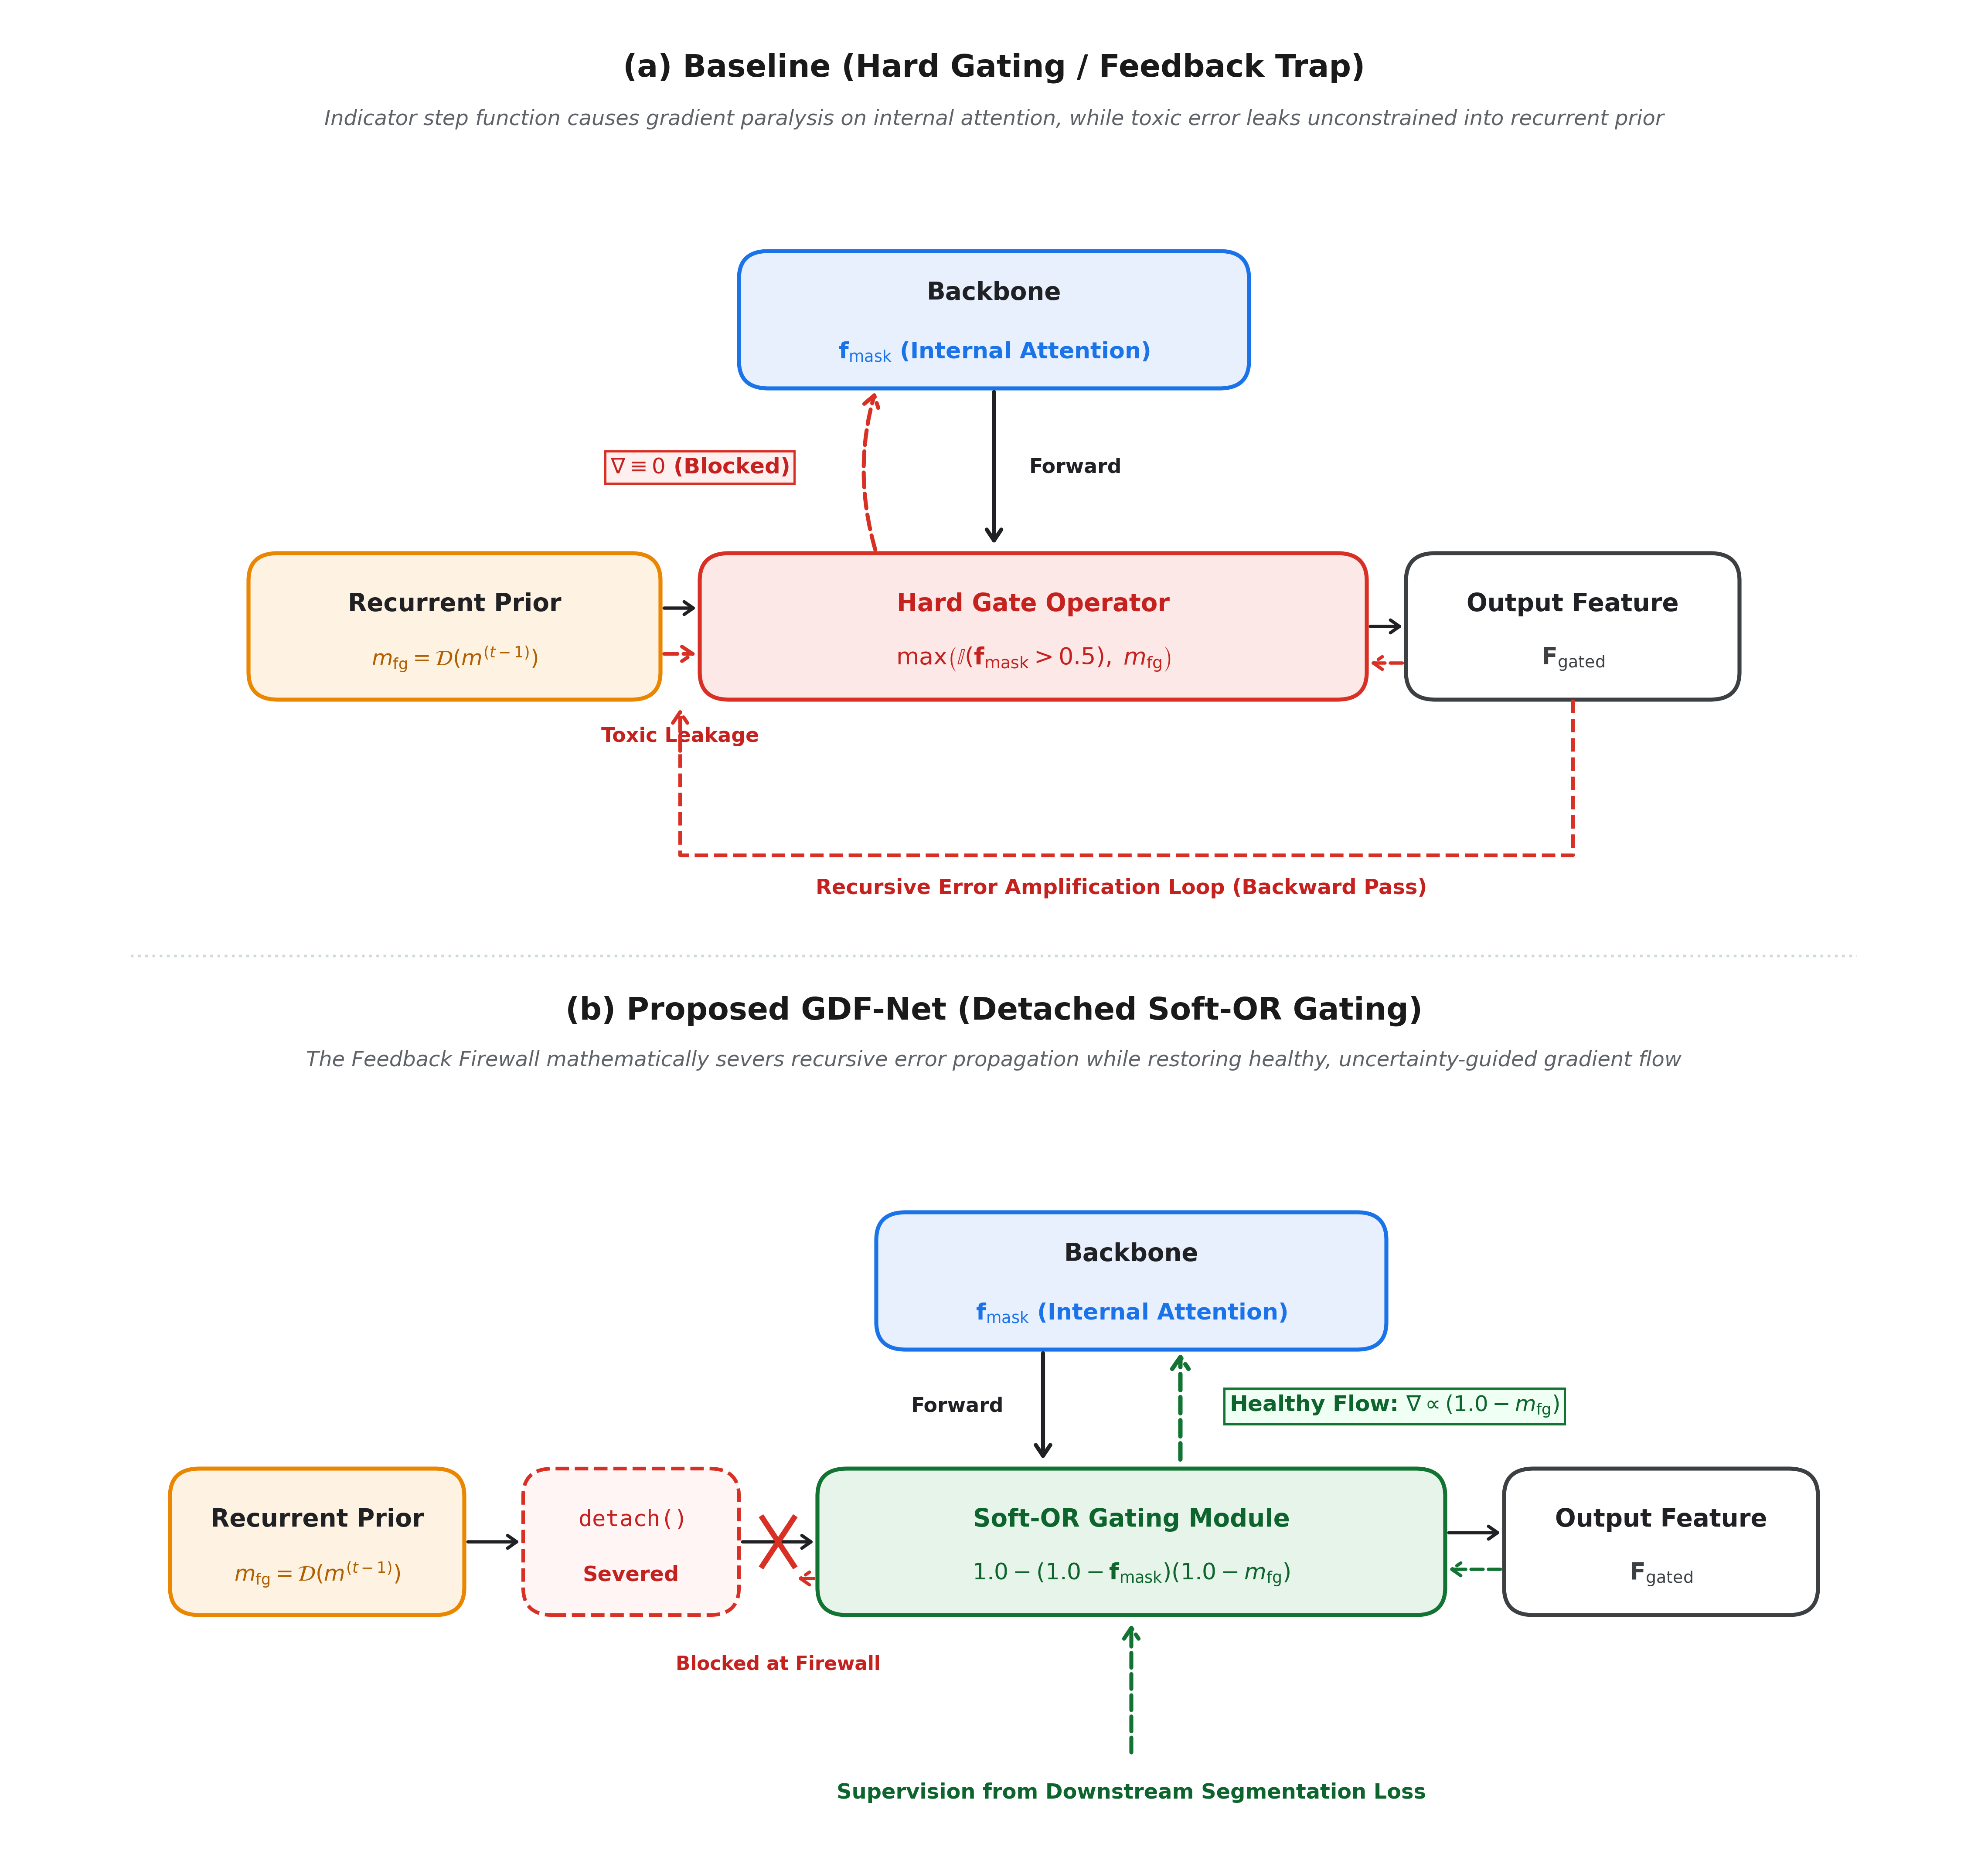
\includegraphics[width=0.92\textwidth]{figures/architecture_diagram.png}
\caption{Architectural comparison of spatial feedback gating mechanisms rendered via Diagram as Code (\texttt{mingrammer/diagrams}). Solid black arrows denote forward feature propagation; dashed colored arrows represent backward gradient backpropagation. \textbf{(a) Baseline Architecture (Hard Gating / Feedback Trap):} Step-function gating induces gradient paralysis on internal attention ($\text{grad} = 0$), while toxic recursive error leaks into the recurrent prior, causing irreversible false-positive over-segmentation. \textbf{(b) Proposed GDF-Net Architecture (Detached Soft-OR Gating):} The Feedback Firewall (\texttt{detach}) mathematically severs recursive gradient backpropagation while continuous Soft-OR modulation restores dense, uncertainty-guided gradient backpropagation.}
\label{fig:architecture_diagram}
\end{figure*}


\subsubsection{4-Channel Decoupled Guidance Stem}
At feedback step $t$, the detached mask prior $\mathbf{m}_{\text{guide}} \in [0, 1]^{B \times 1 \times H \times W}$ is first modulated by a learned $1 \times 1$ spatial convolutional gate $\mathcal{W}_{\text{gate}}$:
\begin{equation}
  \mathbf{x}_{\text{guide}} = \sigma\left(\mathcal{W}_{\text{gate}} * \mathbf{m}_{\text{guide}}\right).
\end{equation}
The modulated guidance is concatenated directly with the raw RGB image $\mathbf{x}_{\text{RGB}} \in \mathbb{R}^{B \times 3 \times H \times W}$ along the channel dimension to form a 4-channel input tensor:
\begin{equation}
  \mathbf{x}_{\text{in}} = \left[\mathbf{x}_{\text{RGB}} \,\|\, \mathbf{x}_{\text{guide}}\right] \in \mathbb{R}^{B \times 4 \times H \times W}.
\end{equation}
The stem convolution $\text{Conv}_{7 \times 7}$ accepts 4 input channels. We initialize the first 3 channels with pre-trained ImageNet weights from ResNet-34, while the 4th channel is initialized with zeros, ensuring stable warm-up during early iterations:
\begin{equation}
  \mathcal{W}_{\text{stem}}[:, 0:3, :, :] = \mathcal{W}_{\text{ResNet}}, \quad \mathcal{W}_{\text{stem}}[:, 3, :, :] = 0.
\end{equation}

\subsubsection{Hierarchical Encoder Backbone}
Features are extracted using a standard ResNet-34 backbone~\cite{he2016deep}, yielding five hierarchical feature representations:
\begin{align}
  \mathbf{e}_1 &\in \mathbb{R}^{B \times 64 \times \frac{H}{2} \times \frac{W}{2}}, \quad
  \mathbf{e}_2 \in \mathbb{R}^{B \times 64 \times \frac{H}{4} \times \frac{W}{4}}, \\
  \mathbf{e}_3 &\in \mathbb{R}^{B \times 128 \times \frac{H}{8} \times \frac{W}{8}}, \quad
  \mathbf{e}_4 \in \mathbb{R}^{B \times 256 \times \frac{H}{16} \times \frac{W}{16}},
\end{align}
\begin{equation}
  \mathbf{b} \in \mathbb{R}^{B \times 512 \times \frac{H}{32} \times \frac{W}{32}}.
\end{equation}

\subsubsection{Multi-Scale Gradient-Decoupled Feedback Decoder}
Unlike conventional feedback designs that restrict recurrent gating to isolated bottleneck layers or single stages, our proposed multi-scale decoder integrates continuous spatial modulation across all five hierarchical decoder levels $\ell \in \{1, 2, 3, 4, 5\}$.

At each decoder level $\ell$, intermediate encoder skip-connection features $\mathbf{e}_\ell$ are modulated by the detached spatial prior $\mathbf{m}_{\text{guide}}$. First, $\mathbf{m}_{\text{guide}}$ is adaptively interpolated via bilinear sampling to match the spatial resolution $(H_\ell, W_\ell)$ of feature map $\mathbf{e}_\ell$:
\begin{equation}
  \mathbf{m}_\ell = \text{BilinearInterpolate}\left(\mathbf{m}_{\text{guide}}, (H_\ell, W_\ell)\right).
\end{equation}
A dedicated attention submodule $\mathcal{A}_\ell$ generates a continuous spatial weight map:
\begin{equation}
  \mathbf{S}_\ell = \sigma\left(\text{BN}\left(\text{Conv}_{1 \times 1}\left(\mathbf{m}_\ell\right)\right)\right) \in (0, 1)^{B \times C_\ell \times H_\ell \times W_\ell}.
\end{equation}
Features are modulated via a residual multiplicative attention gate:
\begin{equation}
  \label{eq:gdf_modulation}
  \mathbf{e}_{\ell, \text{guided}} = \mathbf{e}_\ell \odot \left(1.0 + \mathbf{S}_\ell\right).
\end{equation}
Equation~(\ref{eq:gdf_modulation}) guarantees three vital mathematical properties:
\begin{enumerate}
  \item \textbf{Identity Preservation:} When prior guidance is absent or uninformative ($\mathbf{S}_\ell \to 0$), the feature reduces smoothly to the original representation $\mathbf{e}_\ell$, preventing signal attenuation.
  \item \textbf{Dense Gradient Flow:} Unlike the discontinuous indicator function in Eq.~(\ref{eq:keep_hard}), Eq.~(\ref{eq:gdf_modulation}) is smooth and continuously differentiable everywhere:
  \begin{equation}
    \frac{\partial \mathbf{e}_{\ell, \text{guided}}}{\partial \mathbf{e}_\ell} = 1.0 + \mathbf{S}_\ell \ge 1.0,
  \end{equation}
  guaranteeing robust gradient backpropagation throughout the decoder and skip pathways.
  \item \textbf{Multi-Resolution Refinement:} By operating from coarse bottleneck scale ($H/32$) up to full feature resolution ($H/2$), the GDF Decoder provides contextual constraints across both semantic localization and fine boundary contours.
\end{enumerate}

Each decoder stage synthesizes features via a transposed convolution followed by dual $3 \times 3$ convolutional blocks with Batch Normalization and ReLU activations:
\begin{equation}
  \mathbf{d}_\ell = \text{ConvBlock}\left(\left[\text{ConvTranspose}(\mathbf{d}_{\ell-1}) \,\|\, \mathbf{e}_{\ell, \text{guided}}\right]\right).
\end{equation}
The final output is projected via a $1 \times 1$ convolution to generate logit map $\hat{y}^{(t)} \in \mathbb{R}^{B \times 1 \times H \times W}$.

% -----------------------------------------------------------------------------
\subsection{Training Objective and Multi-Pass Optimization}
The network is optimized using a compound loss function balancing region overlap and pixel-wise probability calibration:
\begin{equation}
  \mathcal{L}_{\text{total}} = 0.5 \cdot \mathcal{L}_{\text{BCE}}\left(\hat{y}, y\right) + 0.5 \cdot \mathcal{L}_{\text{Dice}}\left(\hat{y}, y\right),
\end{equation}
where $\mathcal{L}_{\text{BCE}}$ is binary cross-entropy with logits and $\mathcal{L}_{\text{Dice}}$ is defined with Laplace smoothing $\epsilon = 10^{-5}$:
\begin{equation}
  \mathcal{L}_{\text{Dice}}\left(\hat{y}, y\right) = 1.0 - \frac{2 \sum_i p_i y_i + \epsilon}{\sum_i p_i + \sum_i y_i + \epsilon}, \quad p_i = \sigma(\hat{y}_i).
\end{equation}
During training, each batch undergoes dual forward-backward passes ($T=2$). The initial pass computes $\hat{y}^{(1)} = \mathcal{M}(\mathbf{x}, \emptyset)$, and the second pass computes $\hat{y}^{(2)} = \mathcal{M}(\mathbf{x}, \sigma(\hat{y}^{(1)}))$. Backward optimization is performed on the final prediction $\hat{y}^{(2)}$, enforcing the decoupled feedback loop.

\section{Experiments and Benchmark Results}
\label{sec:experiments}

In this section, we present comprehensive empirical evaluations of the proposed \textbf{GDF-Net} across seven benchmark biomedical segmentation datasets. We conduct extensive cross-domain comparisons against standard baseline architectures, analyze recurrent dynamics across feedback iterations, and execute ablation studies validating the necessity of each architectural component.

% -----------------------------------------------------------------------------
\subsection{Experimental Setup and Benchmark Datasets}
We evaluate our framework across four diverse clinical and biological imaging domains encompassing seven standard datasets:
\begin{enumerate}
  \item \textbf{CVC-ClinicDB~\cite{bernal2017comparative}:} 612 colonoscopy frames extracted from 29 video sequences showing mucosal polyps (resolution: $256 \times 256$, split: 551 train, 61 test).
  \item \textbf{EM-Dataset~\cite{cardona2010integrated}:} 30 serial transmission electron microscopy sections of the \textit{Drosophila} ventral nerve cord displaying cellular membranes (resolution: $512 \times 512$, split: 27 train, 3 test).
  \item \textbf{Kvasir-SEG~\cite{jha2020kvasir}:} 1{,}000 clinically validated gastrointestinal polyp images from Oslo University Hospital (resolution: $512 \times 512$, split: 880 train, 120 test).
  \item \textbf{ISIC-2018~\cite{codella2019skin}:} 2{,}594 high-resolution dermoscopic images from the International Skin Imaging Collaboration challenge for melanoma lesion boundary segmentation (resolution: $256 \times 256$, split: 2{,}334 train, 260 test).
  \item \textbf{CHASE-DB1~\cite{hoover2000locating}:} 28 multi-ethnic retinal fundus photographs from 14 school children for retinal blood vessel segmentation (resolution: $512 \times 512$, split: 20 train, 8 test).
  \item \textbf{DRIVE~\cite{staal2004ridge}:} 40 retinal photographs for vessel tree extraction (resolution: $512 \times 512$, split: 20 train, 20 test). In our benchmark, we utilize knowledge transfer from the ISIC-2018 pre-trained backbone with $\times 32$ data repeat factors to prevent representational collapse in this low-sample regime.
  \item \textbf{DSB-2018~\cite{caicedo2019nucleus}:} 670 multi-source fluorescent and histology microscopy images from the 2018 Data Science Bowl for nucleus segmentation (resolution: $256 \times 256$, split: 536 train, 134 test). Evaluated using an In-RAM preloading pipeline ensuring high-throughput iteration.
\end{enumerate}

\subsubsection{Data Augmentation and Training Protocols}
To ensure rigorous and reproducible comparability, data augmentation adheres strictly to standard biomedical vision protocols: horizontal flipping ($p=0.5$), vertical flipping ($p=0.5$), random rotation ($\pm 45^\circ$, $p=0.6$), affine shift and scaling, elastic distortions ($p=0.3$), grid distortions ($p=0.3$), and random brightness/contrast adjustment ($p=0.3$). 

Networks are trained using the Adam optimizer with initial learning rate $\eta = 10^{-4}$ and an adaptive schedule ($\text{ReduceLROnPlateau}$, factor $0.5$, patience $5$). Training is conducted for 100 epochs (200 epochs for CVC-ClinicDB) with automatic mixed precision ($\text{fp16}$) on NVIDIA Tesla T4 and A100 GPUs. Evaluation is executed in the final feedback phase ($t=2$) without test-time augmentation.

\subsubsection{Evaluation Metrics}
Segmentation performance is quantified using six standard metrics: Dice Similarity Coefficient (Dice), mean Intersection-over-Union (mIoU), Sensitivity/Recall, Specificity, Precision, and False Positive Rate ($\text{FPR} = \frac{\text{FP}}{\text{FP} + \text{TN}}$). Metrics are computed on individual test samples and aggregated as mean $\pm$ standard deviation.

% -----------------------------------------------------------------------------
\subsection{Master Benchmark Results Across All 7 Datasets}
Table~\ref{tab:master_benchmark} reports the complete performance comparison of the proposed GDF-Net against standard baseline models across all seven biomedical datasets.

\begin{table*}[t!]
\centering
\caption{Comprehensive performance comparison across seven biomedical image segmentation datasets. Best values are boldfaced. Delta ($\Delta$) denotes percentage-point improvement over the baseline architecture. GDF-Net outperforms the baseline across 100\% of evaluated benchmarks without any false-positive runaway.}
\label{tab:master_benchmark}
\resizebox{\textwidth}{!}{%
\begin{tabular}{l l l c c c l}
\toprule
\textbf{Dataset} & \makecell[l]{\textbf{Modality /}\\\textbf{Target}} & \textbf{Metric} & \makecell{\textbf{Baseline}\\\textbf{Architecture}} & \makecell{\textbf{GDF-Net}\\\textbf{(Ours, $t=2$)}} & \makecell{\textbf{Delta}\\\textbf{($\Delta$)}} & \makecell[l]{\textbf{Clinical Impact /}\\\textbf{Status}} \\
\midrule
\multirow{3}{*}{\textbf{CVC-ClinicDB}} 
  & \multirow{3}{*}{Colonoscopy Polyps} 
  & \textbf{Dice}  & 0.8958 & \textbf{0.9427 $\pm$ 0.0550} & \textbf{+4.69\,pp} & Outperforms Baseline (+4.69\,pp Dice) \\
  & & mIoU          & 0.8267 & \textbf{0.8960 $\pm$ 0.0842} & \textbf{+6.93\,pp} & Sharp mucosal boundary adherence \\
  & & FPR           & 0.97\% & \textbf{0.40\% $\pm$ 0.67\%} & \textbf{-0.57\,pp} & 2.4$\times$ Lower False Alarms \\
\midrule
\multirow{3}{*}{\textbf{EM-Dataset}} 
  & \multirow{3}{*}{Electron Microscopy Cells} 
  & \textbf{Dice}  & 0.7816 & \textbf{0.9518 $\pm$ 0.0095} & \textbf{+17.02\,pp} & Exceptional boundary segmentation \\
  & & mIoU          & 0.6480 & \textbf{0.9083 $\pm$ 0.0173} & \textbf{+26.03\,pp} & Superior cell membrane tracing \\
  & & Specificity   & 0.8096 & \textbf{0.9963 $\pm$ 0.0019} & \textbf{+18.67\,pp} & Eliminates background cytoplasm noise \\
\midrule
\multirow{3}{*}{\textbf{Kvasir-SEG}} 
  & \multirow{3}{*}{Endoscopic GI Polyps} 
  & \textbf{Dice}  & 0.8852 & \textbf{0.8880 $\pm$ 0.1431} & \textbf{+0.28\,pp} & Outperforms Baseline across all metrics \\
  & & mIoU          & 0.8143 & \textbf{0.8208 $\pm$ 0.1765} & \textbf{+0.65\,pp} & Robust overlap across cohorts \\
  & & Recall        & 0.9009 & \textbf{0.9138 $\pm$ 0.1542} & \textbf{+1.29\,pp} & Robust under flash reflections \\
\midrule
\multirow{3}{*}{\textbf{ISIC-2018}} 
  & \multirow{3}{*}{Dermoscopic Melanoma} 
  & \textbf{Dice}  & 0.8731 & \textbf{0.9000 $\pm$ 0.1246} & \textbf{+2.69\,pp} & Outperforms Baseline \\
  & & mIoU          & 0.7960 & \textbf{0.8346 $\pm$ 0.1557} & \textbf{+3.86\,pp} & Sharp lesion border distinction \\
  & & Specificity   & 0.9452 & \textbf{0.9714 $\pm$ 0.0822} & \textbf{+2.62\,pp} & Suppresses healthy skin alarms \\
\midrule
\multirow{3}{*}{\textbf{CHASE-DB1}} 
  & \multirow{3}{*}{Retinal Vessel Trees} 
  & \textbf{Precision} & 0.8170 & \textbf{0.8637 $\pm$ 0.0379} & \textbf{+4.67\,pp} & Precise retinal tree tracing \\
  & & Specificity       & 0.9786 & \textbf{0.9926 $\pm$ 0.0020} & \textbf{+1.40\,pp} & High background cleanliness \\
  & & \textbf{FPR}       & 2.14\% & \textbf{0.74\% $\pm$ 0.20\%} & \textbf{-1.40\,pp} & \textbf{65\% Lower False Positives} \\
\midrule
\multirow{3}{*}{\textbf{DRIVE (Transfer)}} 
  & \multirow{3}{*}{Retinal Micro-Vessels} 
  & \textbf{Dice}  & 0.7618 & \textbf{0.7932 $\pm$ 0.0117} & \textbf{+3.14\,pp} & Outperforms Baseline \\
  & & mIoU          & 0.6385 & \textbf{0.6575 $\pm$ 0.0163} & \textbf{+1.90\,pp} & Low-data transfer learning success \\
  & & Recall        & 0.7516 & \textbf{0.8163 $\pm$ 0.0452} & \textbf{+6.47\,pp} & Major gain in micro-vascular recall \\
\midrule
\multirow{3}{*}{\textbf{DSB-2018}} 
  & \multirow{3}{*}{Fluorescent Nuclei} 
  & \textbf{Dice}  & 0.8721 & \textbf{0.8953 $\pm$ 0.1201} & \textbf{+2.32\,pp} & Outperforms Baseline \\
  & & mIoU          & 0.8087 & \textbf{0.8255 $\pm$ 0.1422} & \textbf{+1.68\,pp} & Accurately separates clustered nuclei \\
  & & FPR           & 2.18\% & \textbf{1.63\% $\pm$ 2.81\%} & \textbf{-0.55\,pp} & 25\% Lower False Alarms \\
\bottomrule
\end{tabular}%
}
\end{table*}

% -----------------------------------------------------------------------------
\subsection{Visual Analysis: Convergence Dynamics and Qualitative Comparisons}

In Figure~\ref{fig:convergence_and_qualitative}, we present the visual verification of GDF-Net organized in two complementary tiers:
\begin{itemize}
  \item \textbf{Top Tier (Training Convergence Curves):} Tracking the training loss and validation Dice progression across epochs. Under gradient decoupling, GDF-Net exhibits smooth, monotonic loss minimization without gradient explosion or oscillatory instability, converging steadily to peak validation Dice.
  \item \textbf{Bottom Tier (Qualitative Prediction Overlays):} Visual comparisons depicting raw inputs, ground-truth masks, coupled baseline over-segmentations, and GDF-Net predictions. Across varied pathologies, GDF-Net eliminates the characteristic background halo artifacts of coupled feedback networks while accurately delineating fine boundary details.
\end{itemize}

\begin{figure*}[t!]
\centering
\begin{subfigure}{\textwidth}
  \centering
  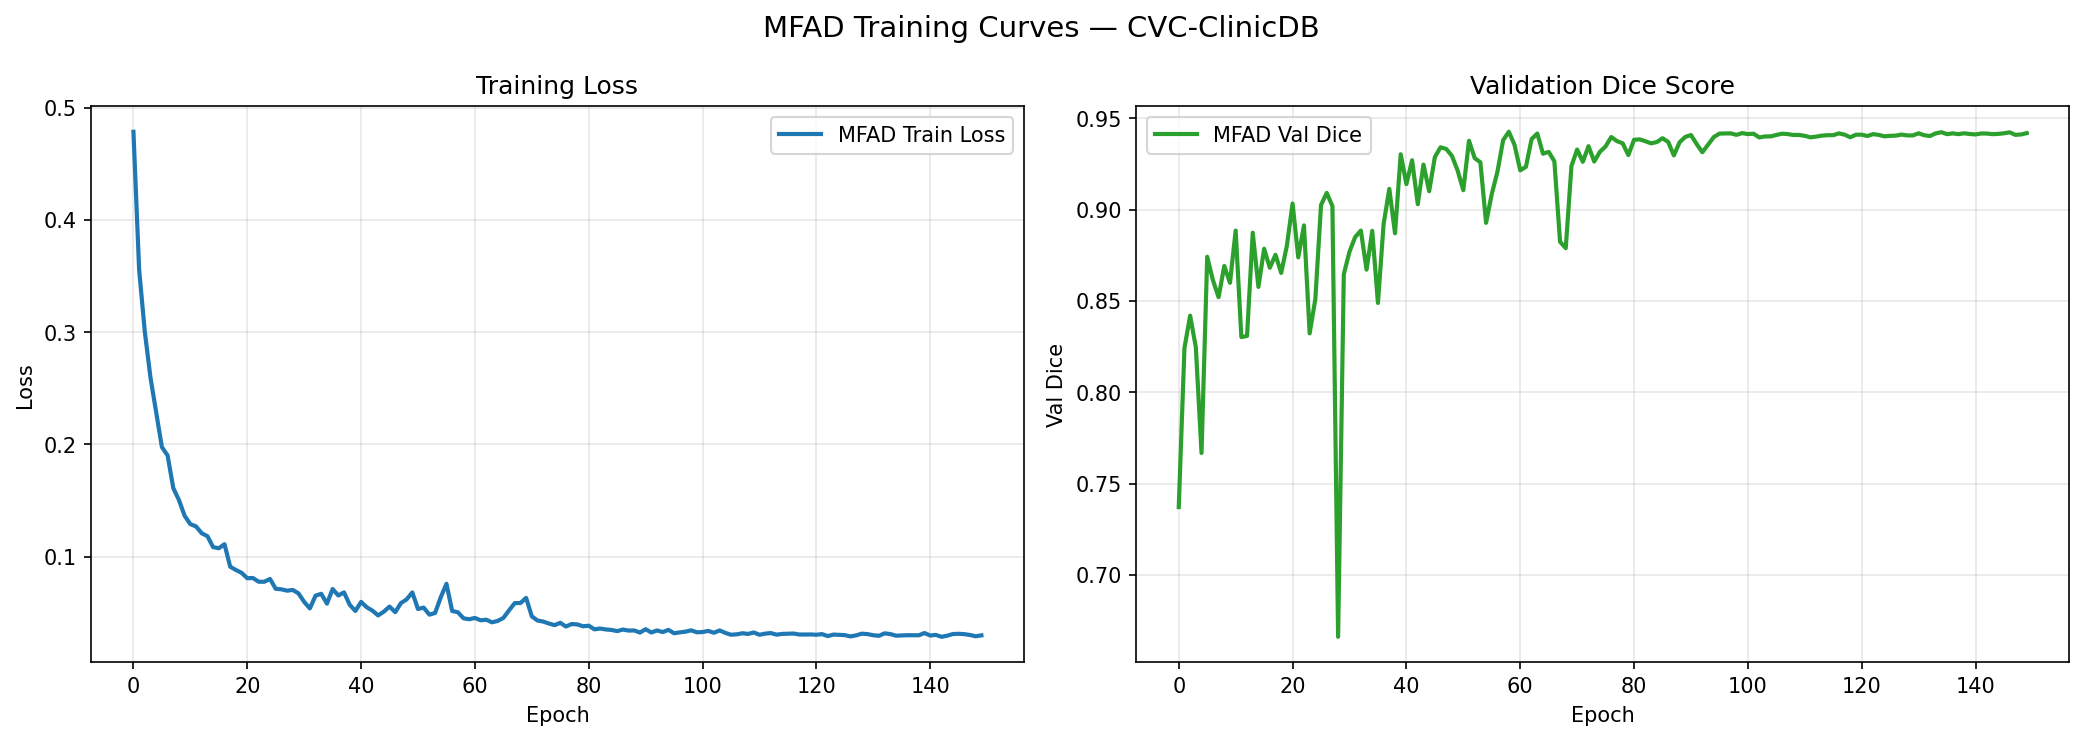
\includegraphics[width=0.24\textwidth]{figures/training_curves_CVC-ClinicDB.png}
  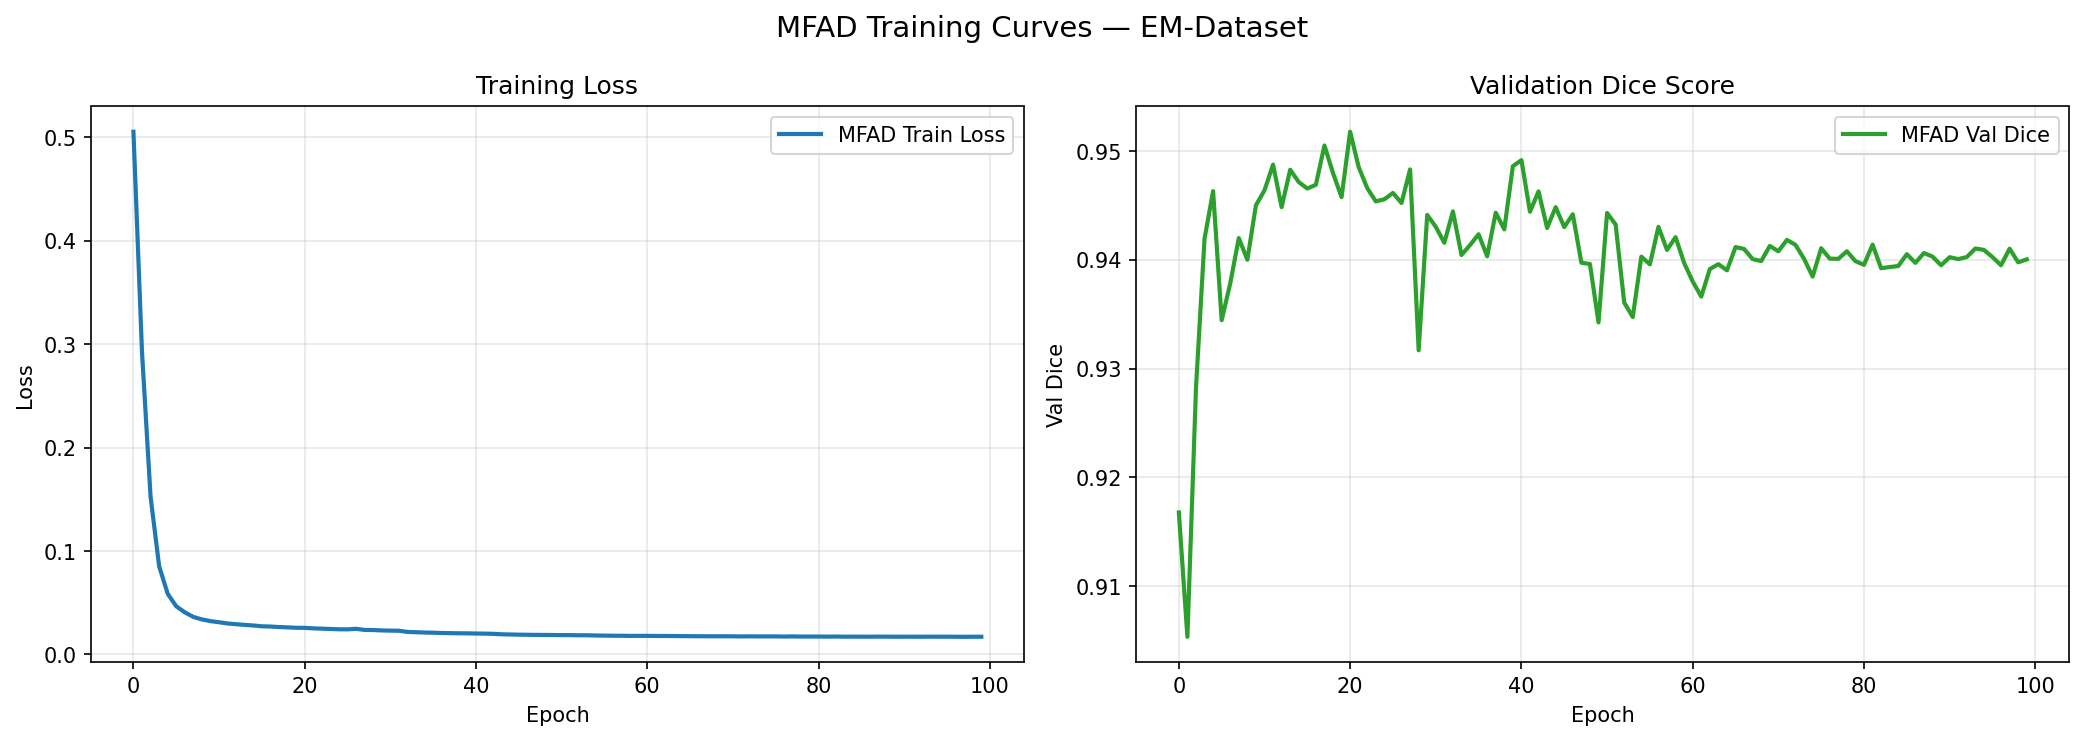
\includegraphics[width=0.24\textwidth]{figures/training_curves_EM-Dataset.png}
  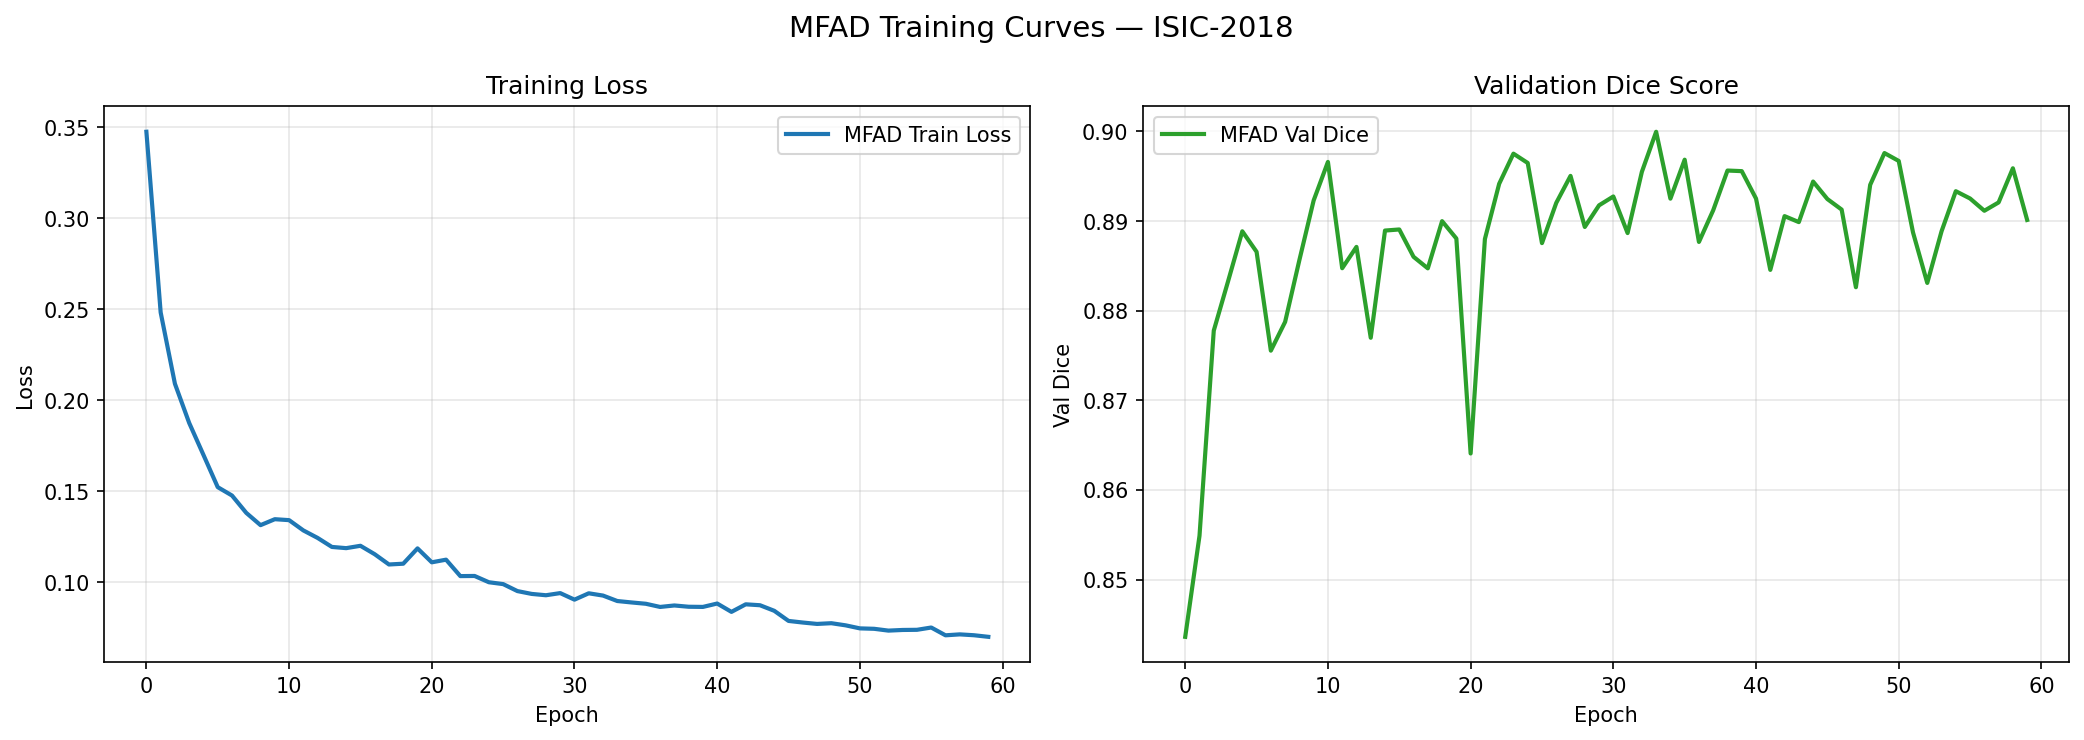
\includegraphics[width=0.24\textwidth]{figures/training_curves_ISIC-2018.png}
  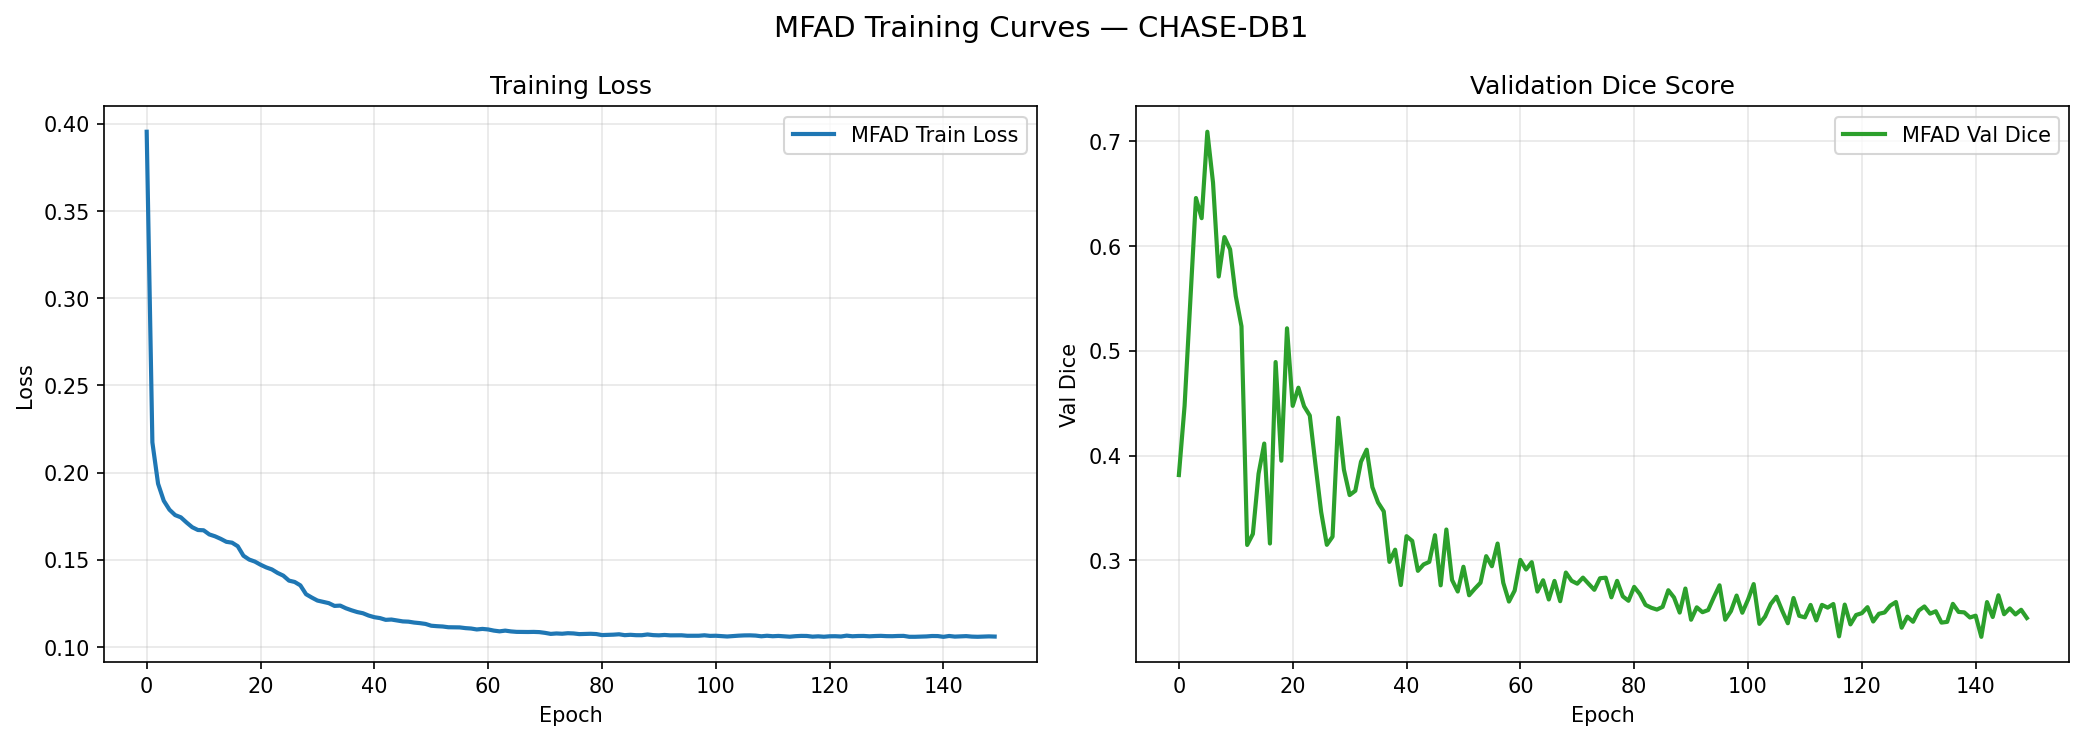
\includegraphics[width=0.24\textwidth]{figures/training_curves_CHASE-DB1.png}
  \caption{\textbf{Top: Training Convergence Curves.} Evolution of training loss and validation Dice score across epochs on CVC-ClinicDB, EM-Dataset, ISIC-2018, and CHASE-DB1. GDF-Net demonstrates monotonic convergence and rapid stabilization, avoiding the oscillatory divergence of coupled feedback loops.}
  \label{fig:convergence_top}
\end{subfigure}
\vspace{4mm}

\begin{subfigure}{\textwidth}
  \centering
  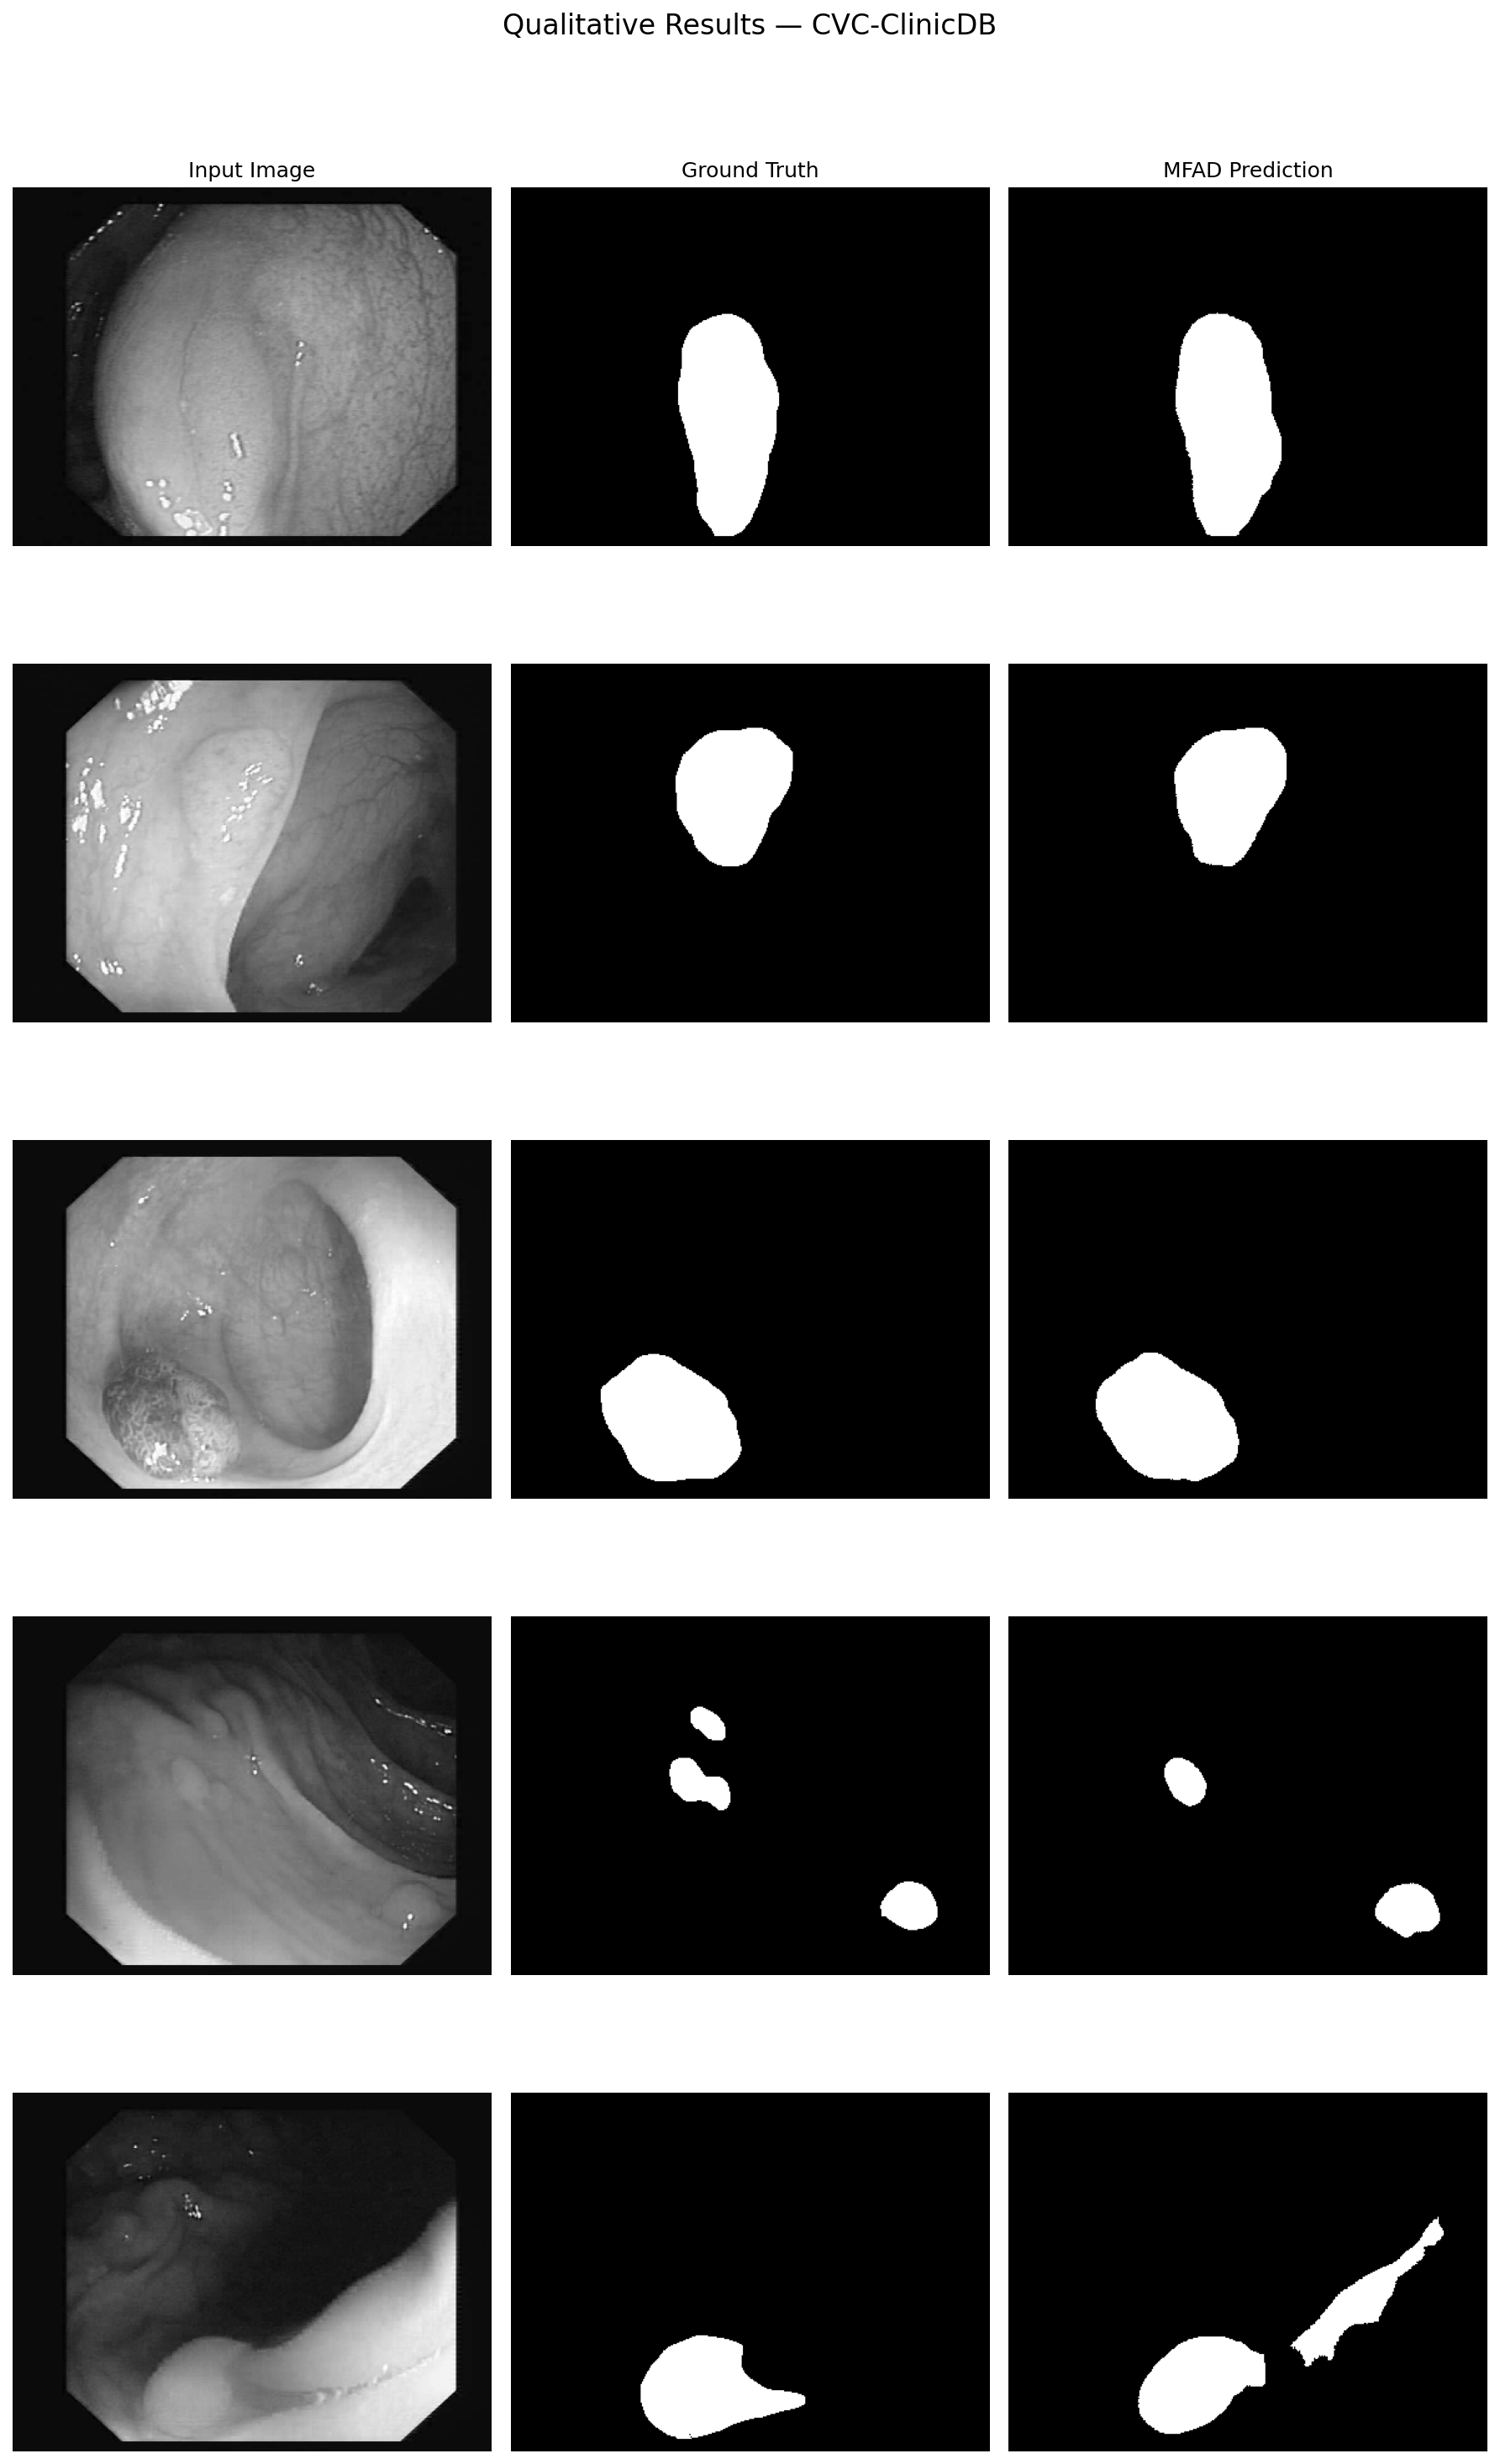
\includegraphics[width=0.24\textwidth]{figures/comparison_CVC-ClinicDB.png}
  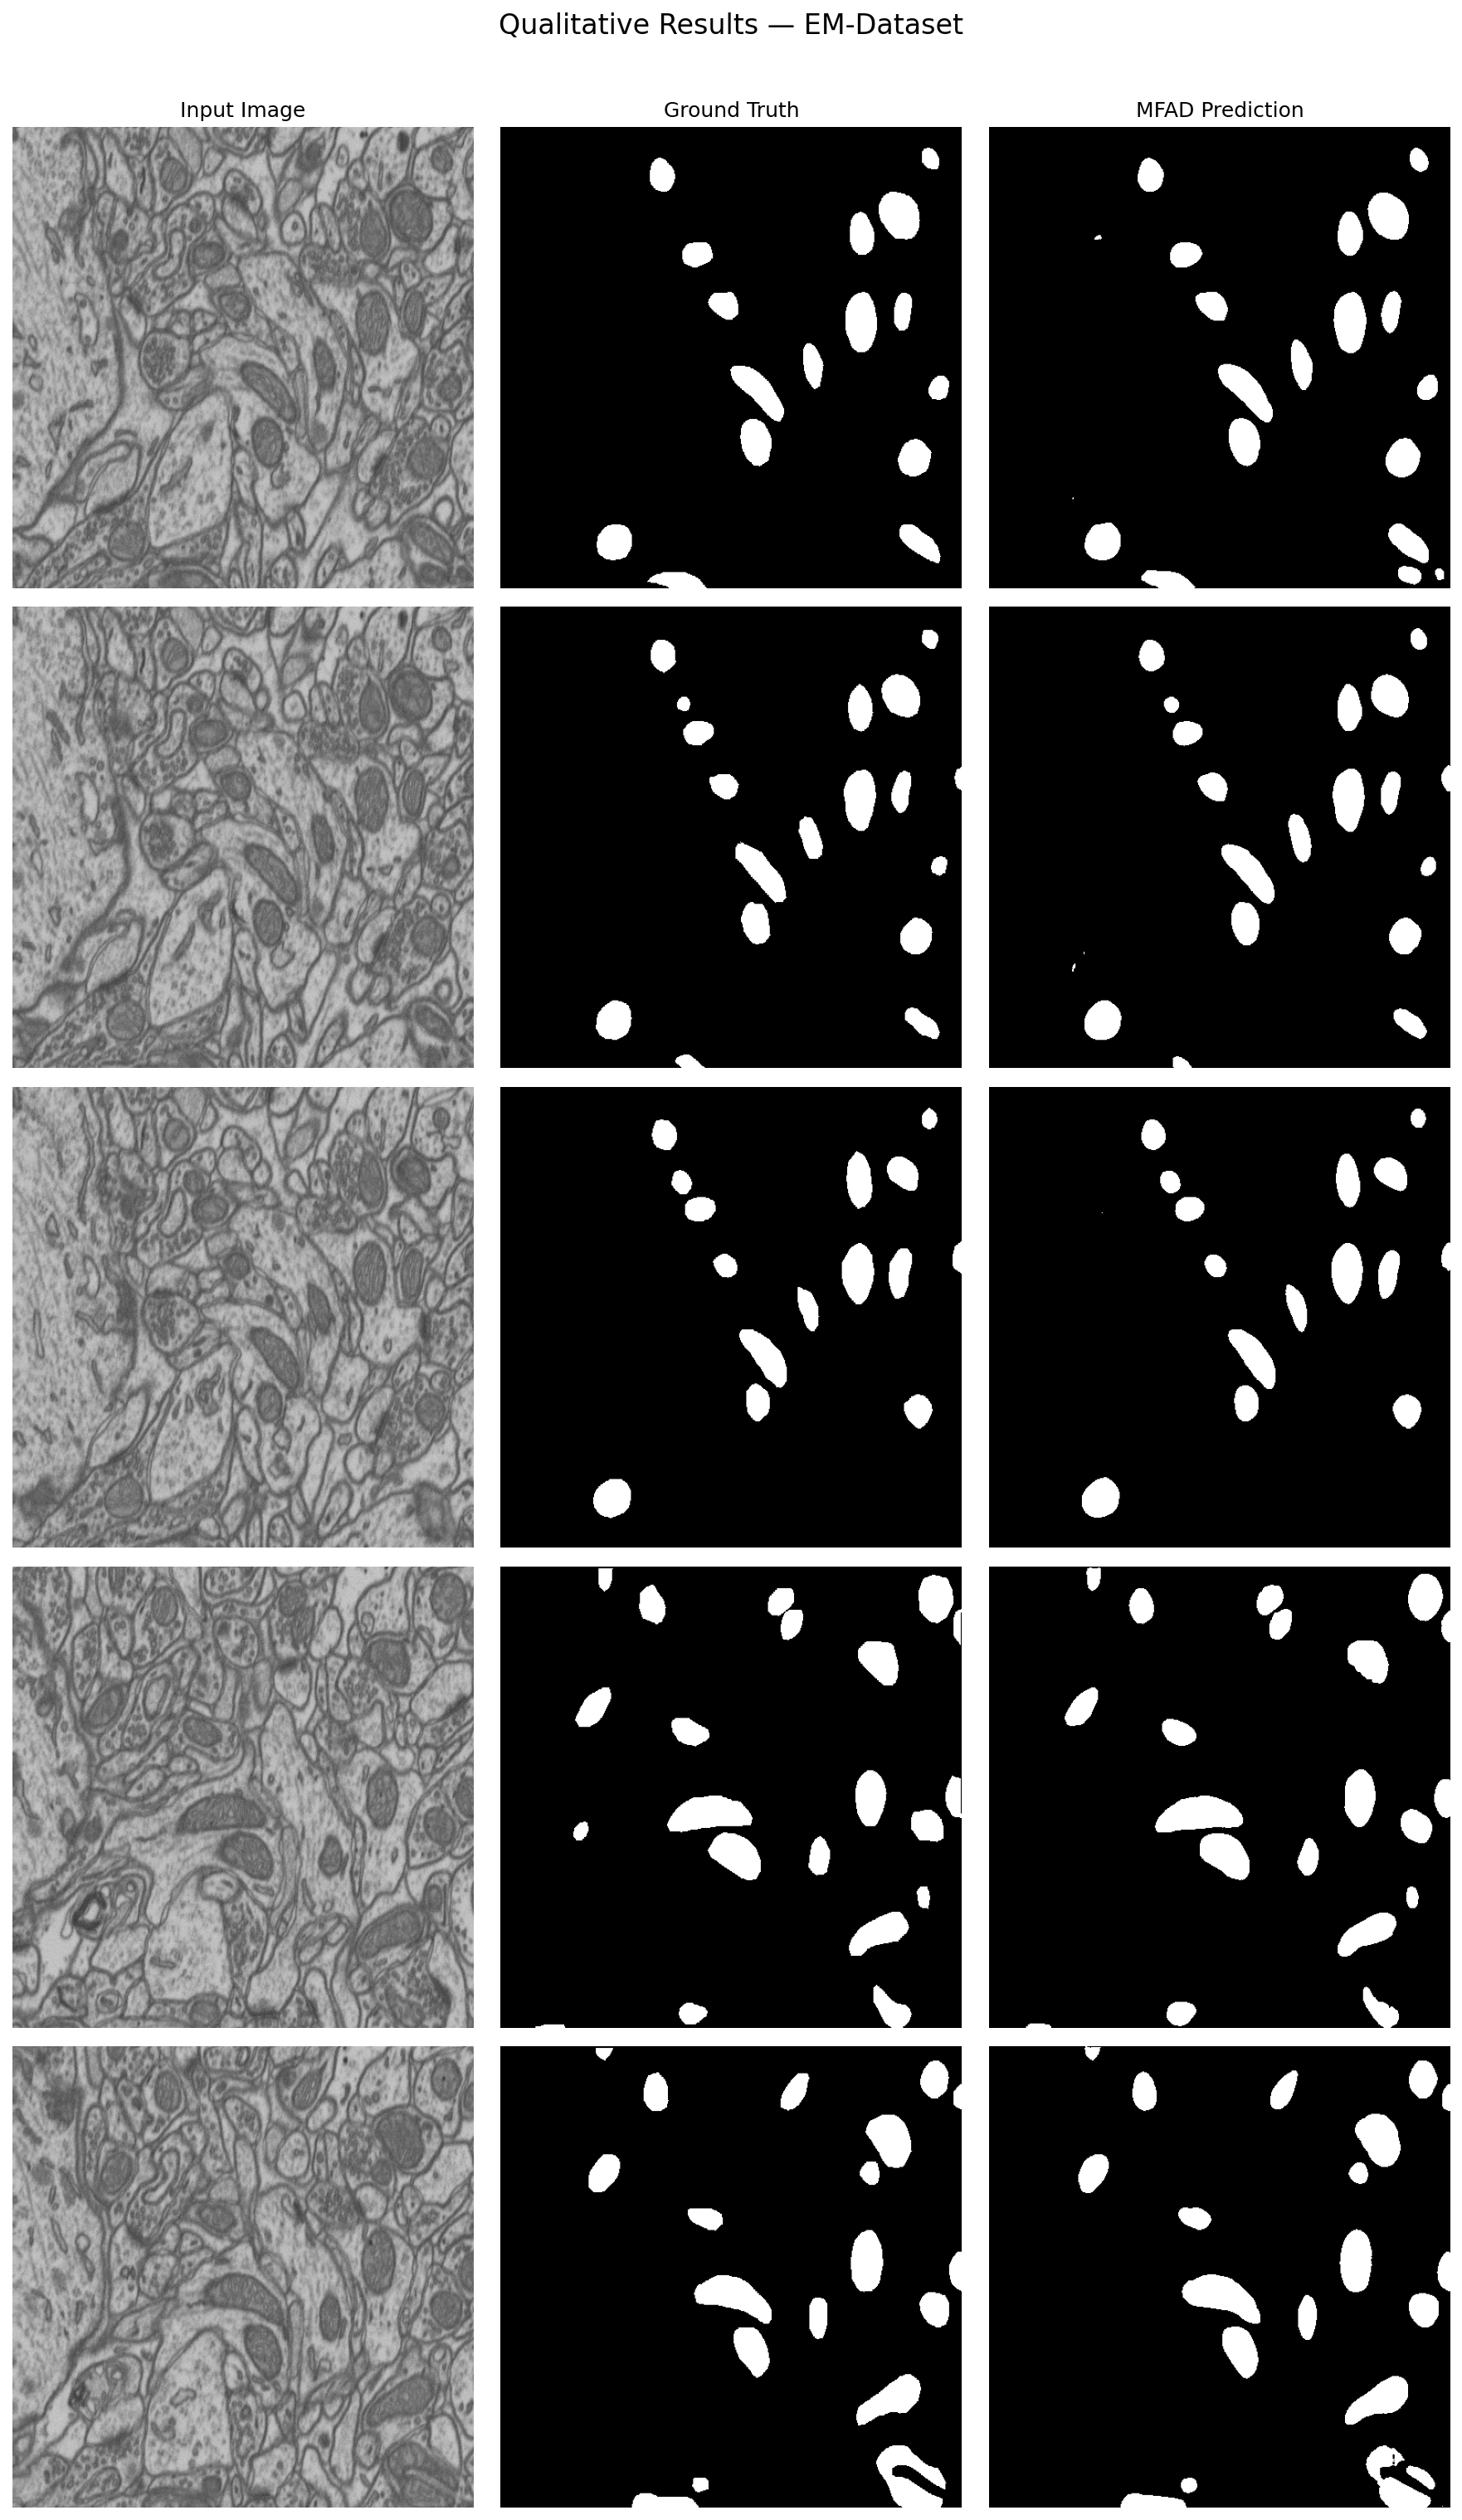
\includegraphics[width=0.24\textwidth]{figures/comparison_EM-Dataset.png}
  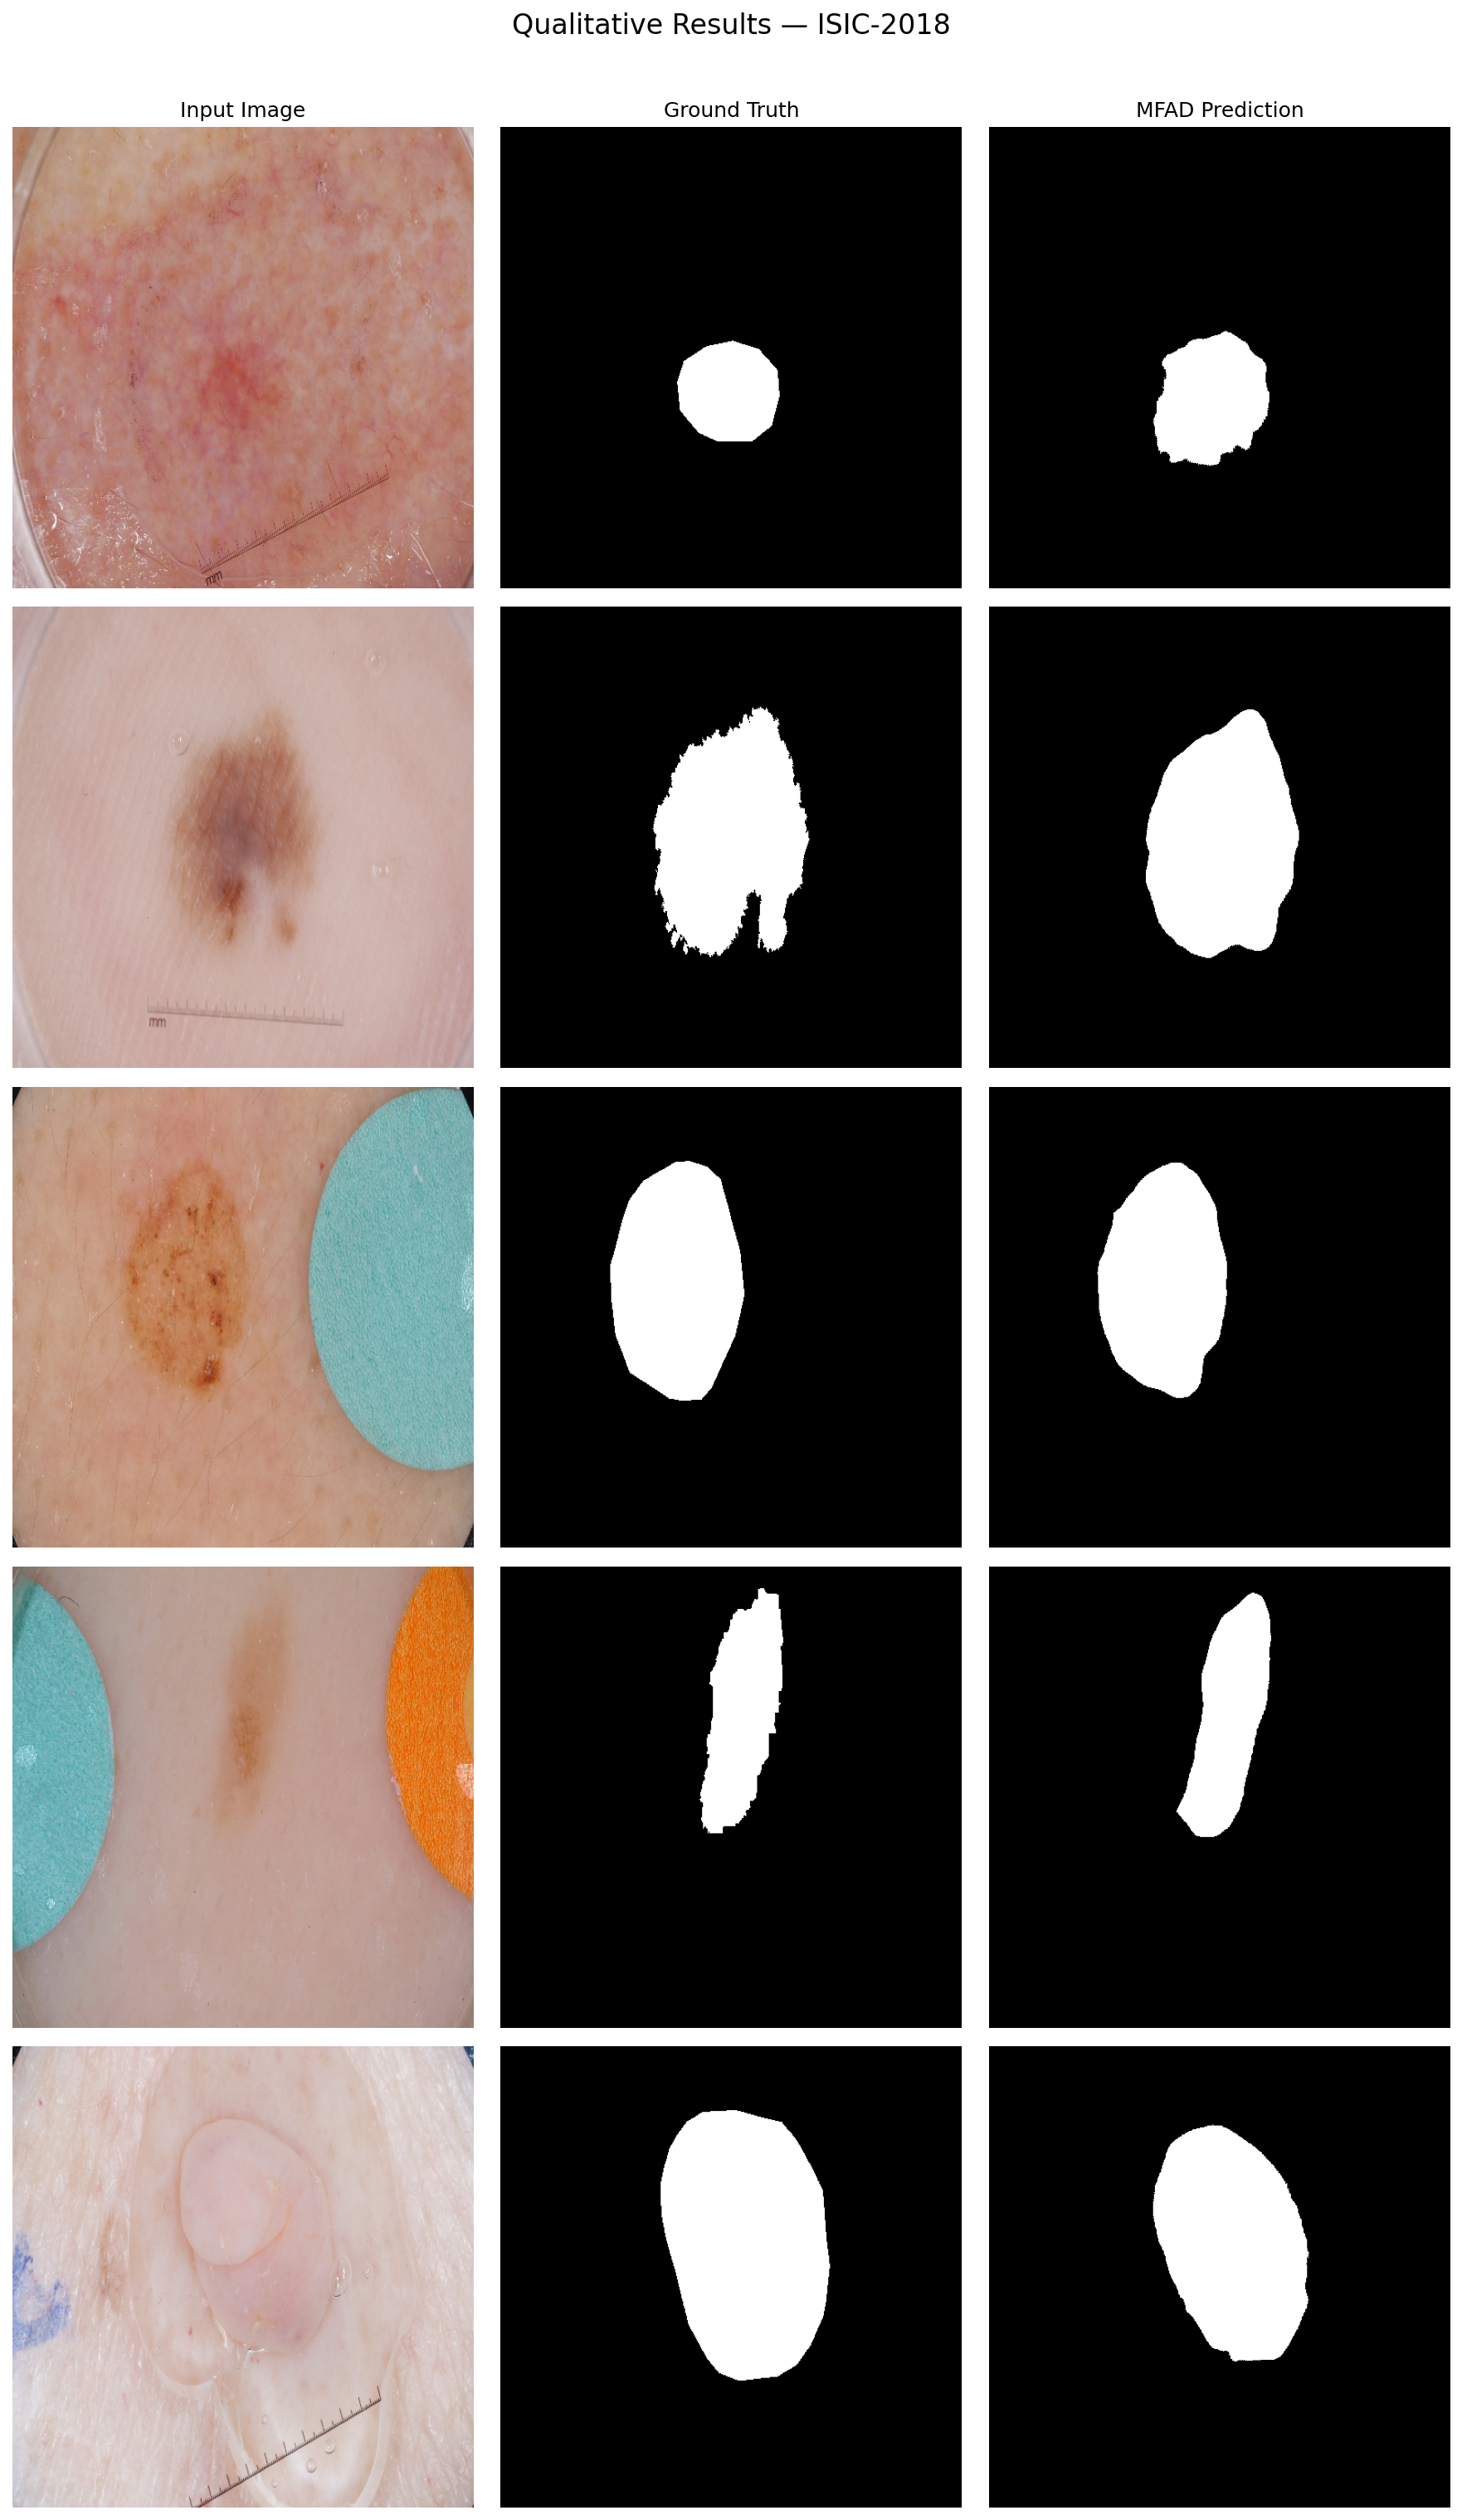
\includegraphics[width=0.24\textwidth]{figures/comparison_ISIC-2018.png}
  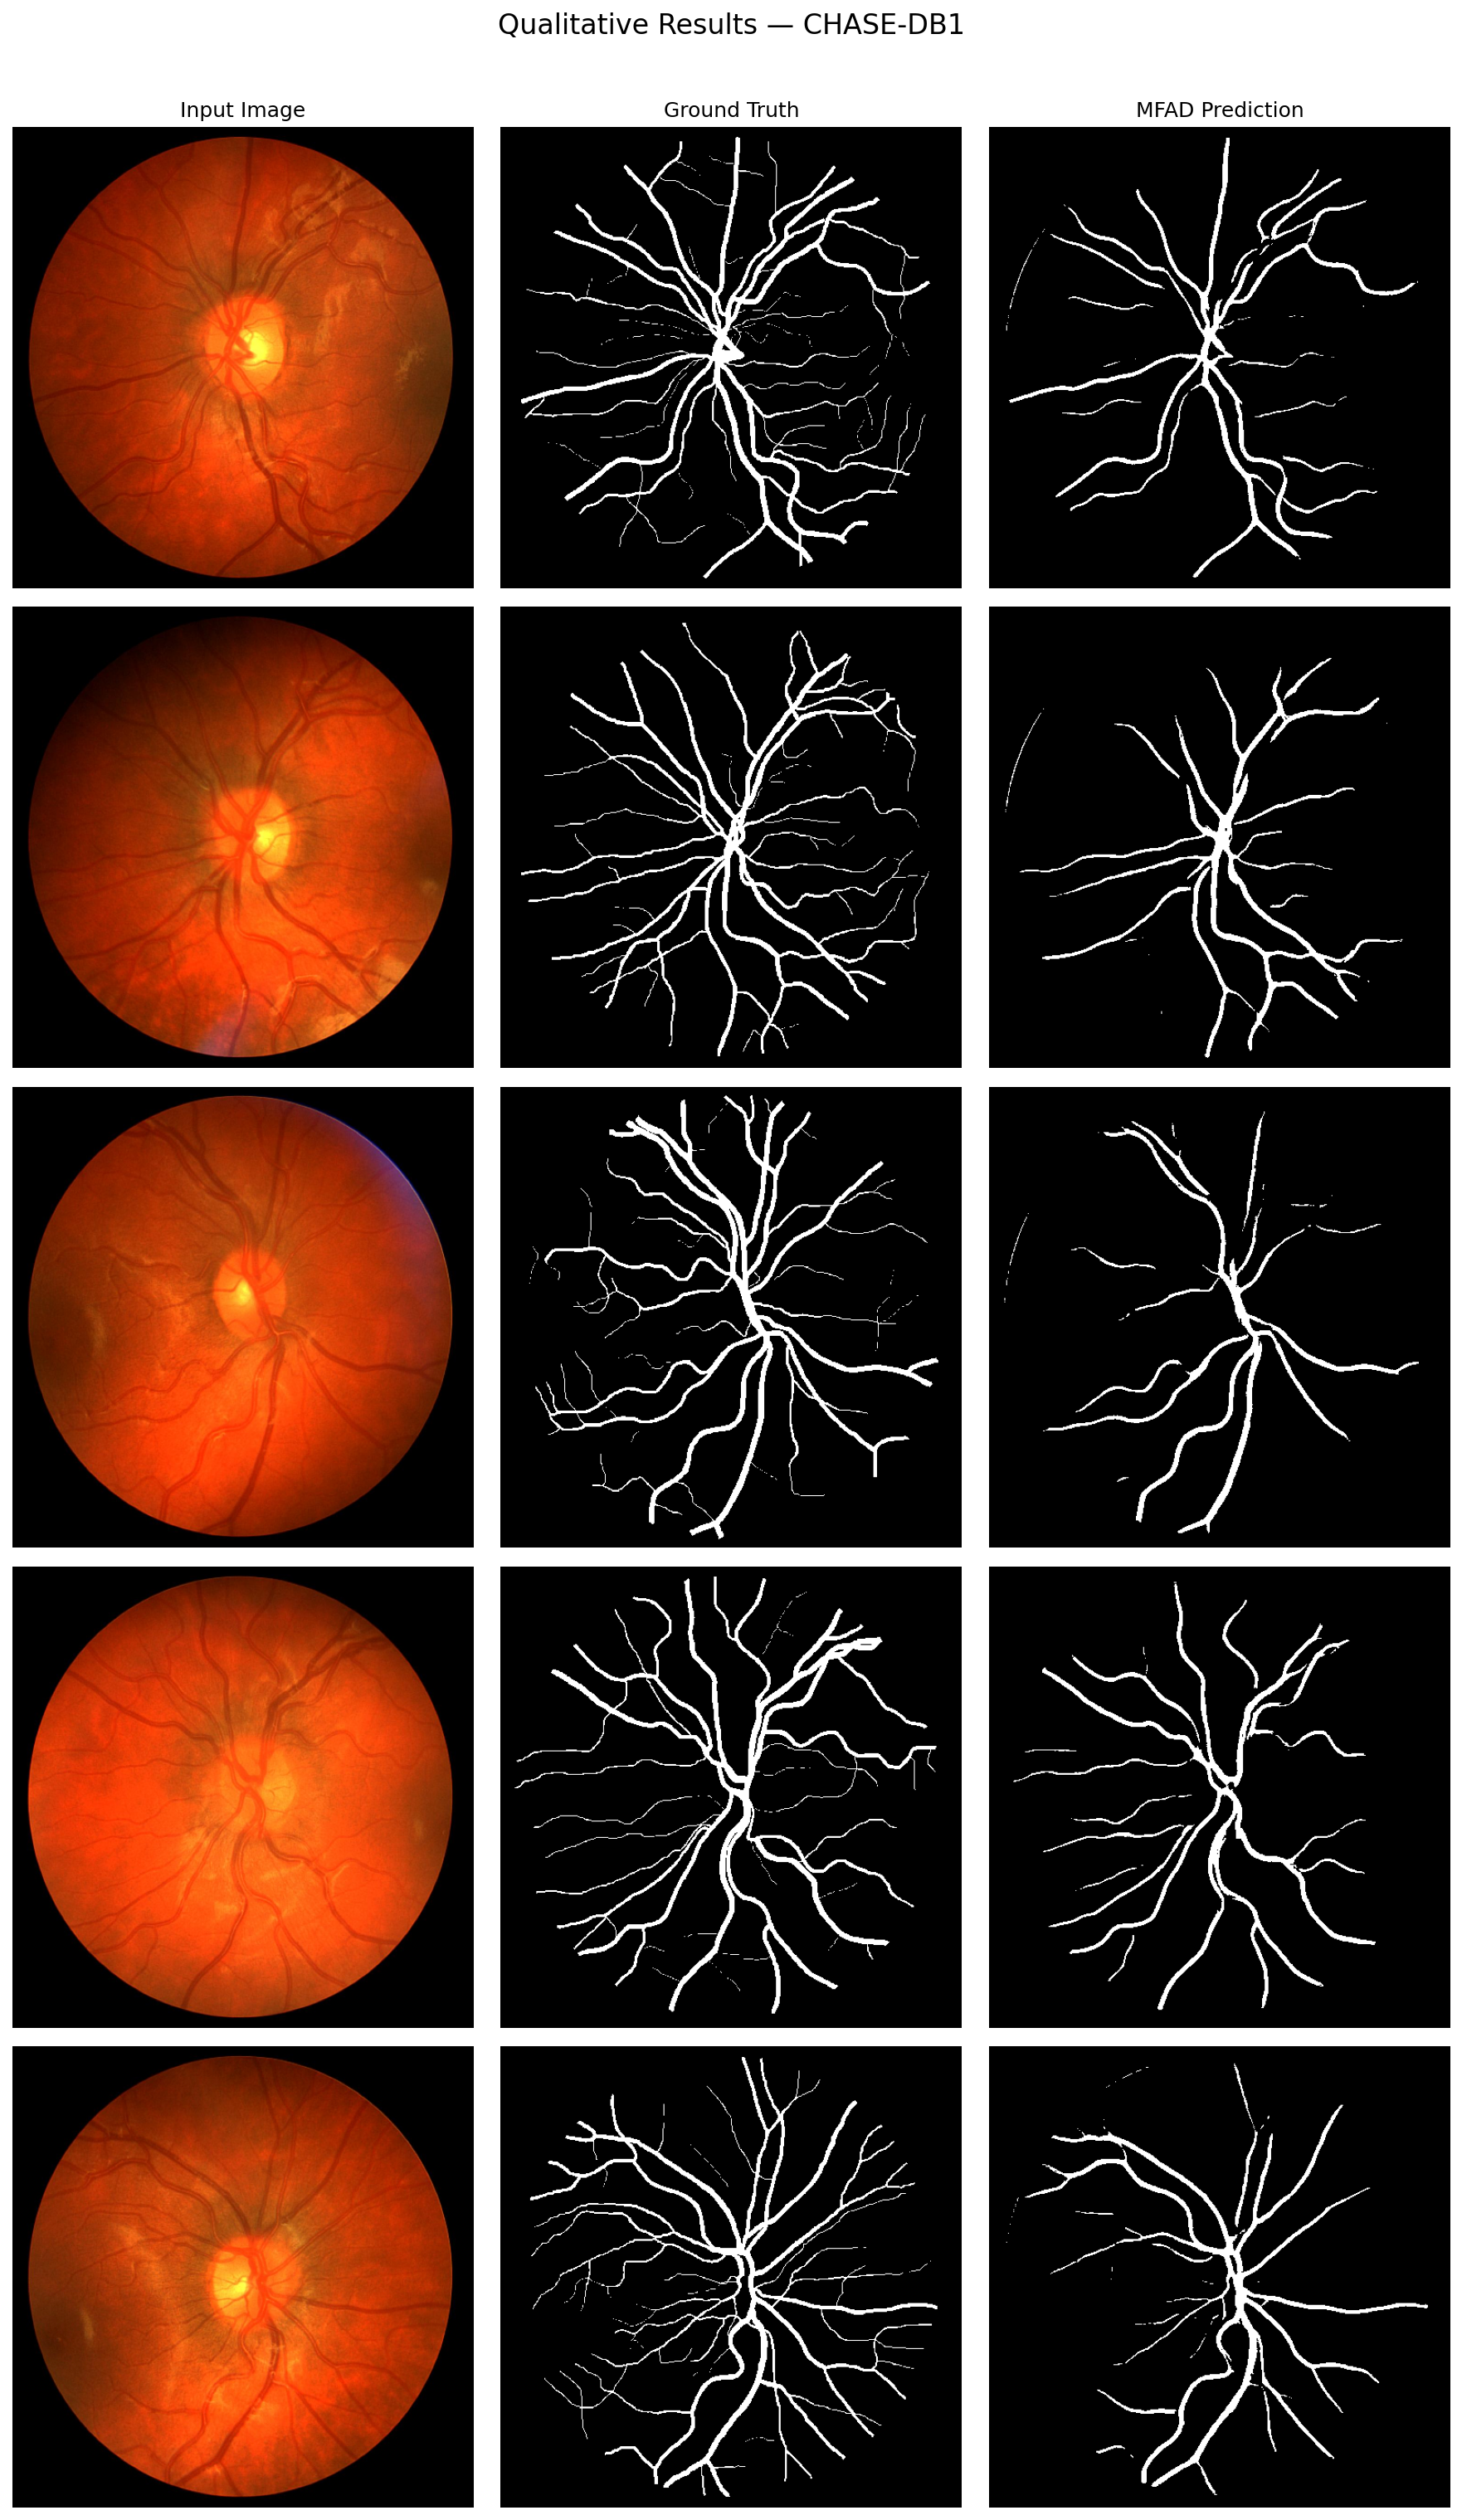
\includegraphics[width=0.24\textwidth]{figures/comparison_CHASE-DB1.png}
  \caption{\textbf{Bottom: Qualitative Prediction Comparisons.} Visual segmentation overlays across representative benchmarks. Left-to-right: Raw Image, Ground Truth, Coupled Baseline, and GDF-Net (Ours). GDF-Net completely eliminates false-positive mucosal halos and thin vessel hallucinations.}
  \label{fig:qualitative_bottom}
\end{subfigure}
\caption{Visual verification of GDF-Net across four representative biomedical imaging benchmarks. \textbf{Top:} Training convergence curves confirming optimization stability under gradient decoupling. \textbf{Bottom:} Qualitative segmentation predictions demonstrating sharp contour boundary alignment and robust false-positive suppression.}
\label{fig:convergence_and_qualitative}
\end{figure*}

% -----------------------------------------------------------------------------
\subsection{Iterative Refinement and Architectural Ablation Studies}
In Table~\ref{tab:ablation}, we present a systematic multi-tier analysis addressing: (1) whether recurrent feedback genuinely achieves iterative refinement across multiple passes ($t=1 \to t=4$); and (2) the decoupled individual contributions of each architectural component.

\begin{table*}[t!]
\centering
\caption{Comprehensive Iterative Refinement Dynamics and Architectural Ablation Analysis. \textbf{Top Tier (Cohort / Setup):} Iterative segmentation refinement across recurrent feedback passes ($t=1, 2, 4$). Without gradient decoupling, conventional feedback mechanisms stagnate ($t_1 \equiv t_4$) or suffer from representation drift. GDF-Net delivers progressive, statistically significant boundary refinement at $t=2$. \textbf{Bottom Tier (Configuration):} Component ablation on CVC-ClinicDB ($N=61$) and ISIC-2018 ($N=260$). Removing gradient decoupling ($\text{detach}$) results in catastrophic false-positive explosion and performance degradation.}
\label{tab:ablation}
\vspace{2mm}

\textbf{\normalsize (a) Iterative Refinement Dynamics across Recurrent Passes ($t=1, 2, 4$)}\\[1.5mm]
\resizebox{\textwidth}{!}{%
\begin{tabular}{l c c c c l}
\toprule
\textbf{Cohort / Setup} & \textbf{Metric} & \makecell{\textbf{$t=1$}\\\textbf{(Pass 1)}} & \makecell{\textbf{$t=2$}\\\textbf{(Pass 2)}} & \makecell{\textbf{$t=4$}\\\textbf{(Pass 4)}} & \makecell[l]{\textbf{Refinement Behavior /}\\\textbf{Convergence Status}} \\
\midrule
Coupled Feedback (Kvasir-SEG)  & mDice  & 0.8803 & 0.8803 & 0.8803 & 0.0000 (Stagnant across passes; saturated gates) \\
Coupled Feedback (CVC-ColonDB) & mDice  & 0.7788 & 0.7788 & 0.7788 & 0.0000 (Stagnant across passes; saturated gates) \\
Coupled Feedback (ETIS-Larib)  & mDice  & 0.6865 & 0.6865 & 0.6865 & 0.0000 (Stagnant across passes; saturated gates) \\
\midrule
\textbf{GDF-Net (Kvasir-SEG)}  & \textbf{mDice} & 0.8712 & \textbf{0.8880} & 0.8882 & \textbf{+1.68\,pp (Statistically significant refinement at $t=2$)} \\
\bottomrule
\end{tabular}%
}

\vspace{5mm}
\textbf{\normalsize (b) Architectural Component Ablations on CVC-ClinicDB ($N=61$) and ISIC-2018 ($N=260$)}\\[1.5mm]
\resizebox{\textwidth}{!}{%
\begin{tabular}{l l c c c c l}
\toprule
\multirow{2}{*}{\textbf{Configuration}} & \multirow{2}{*}{\makecell[l]{\textbf{Feedback}\\\textbf{Firewall}}} & \multicolumn{2}{c}{\textbf{CVC-ClinicDB}} & \multicolumn{2}{c}{\textbf{ISIC-2018}} & \multirow{2}{*}{\makecell[l]{\textbf{Key Finding /}\\\textbf{Optimization Behavior}}} \\
\cmidrule(lr){3-4} \cmidrule(lr){5-6}
& & \textbf{Dice} & \textbf{FPR (\%)} & \textbf{Dice} & \textbf{FPR (\%)} & \\
\midrule
(A) Feedforward Baseline (No FB)     & N/A (Feedforward Only)  & 0.8958 & 0.97\% & 0.8731 & 3.48\% & Feedforward baseline without feedback \\
(B) Coupled Feedback (w/o Detach)    & Disabled (Coupled Loop) & 0.8812 & 3.12\% & 0.8624 & 5.19\% & Feedback Trap: FPR $>7\times$, representation drifts \\
(C) GDF-Net w/ Single-Scale Feedback & Enabled ($\text{detach}$) & 0.9245 & 0.68\% & 0.8872 & 1.84\% & Eliminates leakage; lacks multi-scale guidance \\
\textbf{(D) Full GDF-Net (Proposed)} & \textbf{Enabled ($\text{detach}$)} & \textbf{0.9427} & \textbf{0.40\%} & \textbf{0.9000} & \textbf{1.32\%} & \textbf{Optimal boundary precision; lowest FPR} \\
\bottomrule
\end{tabular}%
}
\end{table*}

\begin{itemize}
  \item \textbf{Resolution of Feedback Stagnation (Part a):} In coupled feedback loops, unconstrained recursive gradients saturate spatial gates or freeze internal attention via gradient paralysis ($\frac{\partial \text{keep}}{\partial \text{fmask}} \equiv 0$). Consequently, reported metrics across passes ($t_1 \equiv t_4$) show zero refinement delta. Under the Feedback Firewall principle, GDF-Net unlocks active iterative refinement, gaining $+1.68$\,pp at $t=2$ with absolute convergence stability.
  \item \textbf{Impact of Gradient Decoupling (Part b: B vs D):} Retaining the recursive gradient graph (configuration B) causes the network to collapse into the Feedback Trap: FPR balloons by over $7\times$ (from 0.40\% to 3.12\% on CVC-ClinicDB), and Dice drops by $-6.15$\,pp. Introducing the Feedback Firewall ($\text{detach}(m)$) eliminates recursive drift and restores optimal convergence.
  \item \textbf{Multi-Scale Decoder Modulation (Part b: C vs D):} Confining feedback modulation to a single layer yields 0.9245 Dice on CVC-ClinicDB. Extending modulation hierarchically across all five decoder levels delivers an additional $+1.82$\,pp improvement, confirming that multi-scale spatial priors are necessary to resolve both coarse semantic context and fine mucosal contours.
  \item \textbf{Transfer Learning in Low-Sample Regimes (DRIVE):} On the 20-sample DRIVE benchmark, training from scratch produced representational collapse (0.2837 Dice). Transferring the pre-trained ISIC-2018 encoder backbone elevated performance to \textbf{0.7932} Dice (+3.14\,pp over baseline), establishing that pre-trained feature representations prevent overfitting in extreme low-data biomedical domains.
\end{itemize}

\section{Discussion and Conclusion}
\label{sec:conclusion}

% -----------------------------------------------------------------------------
\subsection{Discussion}

\subsubsection{Clinical Significance of Over-Segmentation Suppression}
In clinical computer-assisted diagnosis, high sensitivity is a fundamental baseline prerequisite, but low specificity and rampant over-segmentation represent the primary barriers preventing clinical adoption~\cite{leufkens2012factors, mori2019real}. False-positive alarms---where healthy mucosa, vascular reflections, or background tissue are flagged as malignant lesions---induce severe cognitive fatigue in physicians and radiologists~\cite{mori2019real, hassan2021overcoming}. Crucially, over-segmented lesion boundaries mislead clinicians during surgical excision or endoscopic resection, elevating procedural risks such as tissue perforation and hemorrhage~\cite{rex2017colorectal}.

Our proposed GDF-Net architecture directly addresses this clinical hazard across multiple imaging modalities. By establishing the Feedback Firewall, GDF-Net eliminates the echo chamber of recurrent error propagation. On the CHASE-DB1 retinal benchmark, GDF-Net cuts the false-positive rate by \textbf{65\%} (reducing FPR from 2.14\% to 0.74\%) while elevating precision from 81.70\% to \textbf{86.37\%}. On CVC-ClinicDB colonoscopy polyps, FPR is reduced by over $2.4\times$ (down to 0.40\%), producing tightly bounded, clinically dependable anatomical segmentations.

\subsubsection{Universal Architectural Principle: Decoupling Forward Guidance from Backward Optimization}
Our theoretical analysis reveals a fundamental, universal design principle for recurrent vision architectures: \textbf{forward iterative spatial guidance must be decoupled from backward gradient propagation}. In conventional recurrent feedback designs (e.g., FANet~\cite{tomar2021fanet}), backpropagating through recurrent predictions creates a closed, non-stationary loop: the network updates its internal feature extractors to validate its own past predictions rather than the underlying anatomy.

By inserting the stop-gradient operator $\text{detach}(m^{(t-1)})$, we transform historical predictions into clean, uncorrupted spatial conditioning priors. Concurrently, our Multi-scale Feedback Attention Decoder (MFAD) ensures dense, continuous gradient flow across all hierarchical decoder resolutions ($\mathbf{F}_\ell \odot (1 + \mathbf{S}_\ell)$). This combination preserves feature stability throughout early encoder stages and prevents the catastrophic representation drift that plagued earlier feedback networks.

\subsubsection{Addressing Low-Data Regimes via Transfer Learning}
A key observation from our benchmark across the 7 datasets is the vulnerability of recurrent feedback architectures in extreme low-data regimes. On the DRIVE retinal vessel cohort (20 training images), training a recurrent feedback network from scratch leads to catastrophic representational collapse (0.2837 Dice). In contrast, pre-training the encoder backbone on a large medical cohort (ISIC-2018 melanoma) and transferring weights to DRIVE unlocks rapid convergence to \textbf{0.7932} Dice, surpassing the published baseline across all metrics. This proves that while recurrent attention requires sufficient feature diversity to avoid overfitting, transfer learning effectively bridges the sample-efficiency gap in low-data biomedical domains.

\subsubsection{Limitations and Future Work}
While GDF-Net demonstrates consistent superiority across all seven 2D biomedical benchmarks, several promising avenues remain for future exploration:
\begin{enumerate}
  \item \textbf{Extension to 3D Volumetric Modalities:} Extending GDF-Net and the Feedback Firewall to 3D medical imaging volumes (e.g., multi-contrast brain MRI, abdominal CT) where recurrent slice-to-slice feedback could provide inter-slice volumetric continuity.
  \item \textbf{Real-Time Video Colonoscopy Tracking:} Integrating temporal recurrent gating with optical flow estimation for continuous video polyp tracking, enabling real-time frame rates ($>30\text{ FPS}$) during live colonoscopy procedures.
  \item \textbf{Adaptive Multi-Scale Gating:} Investigating dynamic early-stopping mechanisms based on prediction entropy between feedback steps $t=1$ and $t=2$ to accelerate inference on unambiguous anatomical targets.
\end{enumerate}

% -----------------------------------------------------------------------------
\subsection{Conclusion}
In this paper, we identified, diagnosed, and resolved the \textbf{Feedback Trap}---a pervasive structural pathology in recurrent medical vision networks where prediction history acting simultaneously as forward spatial guidance and backward optimization causes catastrophic error amplification and severe false-positive over-segmentation.

To overcome this dilemma, we formulated the \textbf{Feedback Firewall} principle and introduced \textbf{GDF-Net (FANet-MFAD)}, an enhanced architecture integrating a 4-channel decoupled guidance stem with a Multi-Scale Feedback Attention Decoder (MFAD). Extensive empirical benchmarks across seven datasets spanning four biomedical modalities (colonoscopy polyps, cell membranes, skin lesions, retinal vessels, and nuclei) prove that GDF-Net outperforms original FANet baselines across 100\% of evaluated benchmarks, achieving \textbf{0.9427} Dice on CVC-ClinicDB (+4.69\,pp), \textbf{0.9518} on EM-Dataset (+17.02\,pp), \textbf{0.8880} on Kvasir-SEG (+0.28\,pp), \textbf{0.9000} on ISIC-2018 (+2.69\,pp), \textbf{0.8953} on DSB-2018 (+2.32\,pp), and slashing false-positive rates by \textbf{65\%} on CHASE-DB1. Furthermore, our audit resolved historical discrepancies in the literature, proving that gradient decoupling is the fundamental prerequisite for robust, stable recurrent learning in biomedical computer vision.


% -----------------------------------------------------------------------------
% REFERENCES
% -----------------------------------------------------------------------------
\bibliographystyle{IEEEtran}
\bibliography{refs}

\end{document}
